% Options for packages loaded elsewhere
\PassOptionsToPackage{unicode}{hyperref}
\PassOptionsToPackage{hyphens}{url}
\PassOptionsToPackage{dvipsnames,svgnames,x11names}{xcolor}
%
\documentclass[
  letterpaper,
  DIV=11,
  numbers=noendperiod]{scrartcl}

\usepackage{amsmath,amssymb}
\usepackage{iftex}
\ifPDFTeX
  \usepackage[T1]{fontenc}
  \usepackage[utf8]{inputenc}
  \usepackage{textcomp} % provide euro and other symbols
\else % if luatex or xetex
  \usepackage{unicode-math}
  \defaultfontfeatures{Scale=MatchLowercase}
  \defaultfontfeatures[\rmfamily]{Ligatures=TeX,Scale=1}
\fi
\usepackage{lmodern}
\ifPDFTeX\else  
    % xetex/luatex font selection
\fi
% Use upquote if available, for straight quotes in verbatim environments
\IfFileExists{upquote.sty}{\usepackage{upquote}}{}
\IfFileExists{microtype.sty}{% use microtype if available
  \usepackage[]{microtype}
  \UseMicrotypeSet[protrusion]{basicmath} % disable protrusion for tt fonts
}{}
\makeatletter
\@ifundefined{KOMAClassName}{% if non-KOMA class
  \IfFileExists{parskip.sty}{%
    \usepackage{parskip}
  }{% else
    \setlength{\parindent}{0pt}
    \setlength{\parskip}{6pt plus 2pt minus 1pt}}
}{% if KOMA class
  \KOMAoptions{parskip=half}}
\makeatother
\usepackage{xcolor}
\ifLuaTeX
  \usepackage{luacolor}
  \usepackage[soul]{lua-ul}
\else
  \usepackage{soul}
  
\fi
\setlength{\emergencystretch}{3em} % prevent overfull lines
\setcounter{secnumdepth}{-\maxdimen} % remove section numbering
% Make \paragraph and \subparagraph free-standing
\makeatletter
\ifx\paragraph\undefined\else
  \let\oldparagraph\paragraph
  \renewcommand{\paragraph}{
    \@ifstar
      \xxxParagraphStar
      \xxxParagraphNoStar
  }
  \newcommand{\xxxParagraphStar}[1]{\oldparagraph*{#1}\mbox{}}
  \newcommand{\xxxParagraphNoStar}[1]{\oldparagraph{#1}\mbox{}}
\fi
\ifx\subparagraph\undefined\else
  \let\oldsubparagraph\subparagraph
  \renewcommand{\subparagraph}{
    \@ifstar
      \xxxSubParagraphStar
      \xxxSubParagraphNoStar
  }
  \newcommand{\xxxSubParagraphStar}[1]{\oldsubparagraph*{#1}\mbox{}}
  \newcommand{\xxxSubParagraphNoStar}[1]{\oldsubparagraph{#1}\mbox{}}
\fi
\makeatother


\providecommand{\tightlist}{%
  \setlength{\itemsep}{0pt}\setlength{\parskip}{0pt}}\usepackage{longtable,booktabs,array}
\usepackage{calc} % for calculating minipage widths
% Correct order of tables after \paragraph or \subparagraph
\usepackage{etoolbox}
\makeatletter
\patchcmd\longtable{\par}{\if@noskipsec\mbox{}\fi\par}{}{}
\makeatother
% Allow footnotes in longtable head/foot
\IfFileExists{footnotehyper.sty}{\usepackage{footnotehyper}}{\usepackage{footnote}}
\makesavenoteenv{longtable}
\usepackage{graphicx}
\makeatletter
\newsavebox\pandoc@box
\newcommand*\pandocbounded[1]{% scales image to fit in text height/width
  \sbox\pandoc@box{#1}%
  \Gscale@div\@tempa{\textheight}{\dimexpr\ht\pandoc@box+\dp\pandoc@box\relax}%
  \Gscale@div\@tempb{\linewidth}{\wd\pandoc@box}%
  \ifdim\@tempb\p@<\@tempa\p@\let\@tempa\@tempb\fi% select the smaller of both
  \ifdim\@tempa\p@<\p@\scalebox{\@tempa}{\usebox\pandoc@box}%
  \else\usebox{\pandoc@box}%
  \fi%
}
% Set default figure placement to htbp
\def\fps@figure{htbp}
\makeatother
% definitions for citeproc citations
\NewDocumentCommand\citeproctext{}{}
\NewDocumentCommand\citeproc{mm}{%
  \begingroup\def\citeproctext{#2}\cite{#1}\endgroup}
\makeatletter
 % allow citations to break across lines
 \let\@cite@ofmt\@firstofone
 % avoid brackets around text for \cite:
 \def\@biblabel#1{}
 \def\@cite#1#2{{#1\if@tempswa , #2\fi}}
\makeatother
\newlength{\cslhangindent}
\setlength{\cslhangindent}{1.5em}
\newlength{\csllabelwidth}
\setlength{\csllabelwidth}{3em}
\newenvironment{CSLReferences}[2] % #1 hanging-indent, #2 entry-spacing
 {\begin{list}{}{%
  \setlength{\itemindent}{0pt}
  \setlength{\leftmargin}{0pt}
  \setlength{\parsep}{0pt}
  % turn on hanging indent if param 1 is 1
  \ifodd #1
   \setlength{\leftmargin}{\cslhangindent}
   \setlength{\itemindent}{-1\cslhangindent}
  \fi
  % set entry spacing
  \setlength{\itemsep}{#2\baselineskip}}}
 {\end{list}}
\usepackage{calc}
\newcommand{\CSLBlock}[1]{\hfill\break\parbox[t]{\linewidth}{\strut\ignorespaces#1\strut}}
\newcommand{\CSLLeftMargin}[1]{\parbox[t]{\csllabelwidth}{\strut#1\strut}}
\newcommand{\CSLRightInline}[1]{\parbox[t]{\linewidth - \csllabelwidth}{\strut#1\strut}}
\newcommand{\CSLIndent}[1]{\hspace{\cslhangindent}#1}

\KOMAoption{captions}{tableheading,figureheading}
\makeatletter
\@ifpackageloaded{caption}{}{\usepackage{caption}}
\AtBeginDocument{%
\ifdefined\contentsname
  \renewcommand*\contentsname{Table of contents}
\else
  \newcommand\contentsname{Table of contents}
\fi
\ifdefined\listfigurename
  \renewcommand*\listfigurename{List of Figures}
\else
  \newcommand\listfigurename{List of Figures}
\fi
\ifdefined\listtablename
  \renewcommand*\listtablename{List of Tables}
\else
  \newcommand\listtablename{List of Tables}
\fi
\ifdefined\figurename
  \renewcommand*\figurename{Figure}
\else
  \newcommand\figurename{Figure}
\fi
\ifdefined\tablename
  \renewcommand*\tablename{Table}
\else
  \newcommand\tablename{Table}
\fi
}
\@ifpackageloaded{float}{}{\usepackage{float}}
\floatstyle{ruled}
\@ifundefined{c@chapter}{\newfloat{codelisting}{h}{lop}}{\newfloat{codelisting}{h}{lop}[chapter]}
\floatname{codelisting}{Listing}
\newcommand*\listoflistings{\listof{codelisting}{List of Listings}}
\makeatother
\makeatletter
\makeatother
\makeatletter
\@ifpackageloaded{caption}{}{\usepackage{caption}}
\@ifpackageloaded{subcaption}{}{\usepackage{subcaption}}
\makeatother

\usepackage{bookmark}

\IfFileExists{xurl.sty}{\usepackage{xurl}}{} % add URL line breaks if available
\urlstyle{same} % disable monospaced font for URLs
\hypersetup{
  pdftitle={A Process for Emulating Comparative Oncology Trials with Real-world Evidence Studies (ENCORE): Process Development and Methodological Considerations for Oncology Real-World Data},
  colorlinks=true,
  linkcolor={blue},
  filecolor={Maroon},
  citecolor={Blue},
  urlcolor={Blue},
  pdfcreator={LaTeX via pandoc}}


\title{A Process for Emulating Comparative Oncology Trials with
Real-world Evidence Studies (ENCORE): Process Development and
Methodological Considerations for Oncology Real-World Data}
\author{}
\date{}

\begin{document}
\maketitle


\textbf{Authors}: Janick Weberpals\textsuperscript{1}, Kenneth L.
Kehl\textsuperscript{2}, Donna R. Rivera\textsuperscript{3}, Pallavi
Mishra-Kalyani\textsuperscript{3}, Catherine C.
Lerro\textsuperscript{3}, Erin Larkins\textsuperscript{4}, Sonia
Singh\textsuperscript{4}, Preeti Narayan\textsuperscript{4}, Richard
Curley\textsuperscript{4}, Paul Kluetz\textsuperscript{4}, Georg
Hahn\textsuperscript{1}, Priyanka Anand\textsuperscript{1}, Yanina
Natanzon\textsuperscript{5}, Andrew J. Belli\textsuperscript{6},
Ching-Kun Wang\textsuperscript{6}, Jenna
Collins\textsuperscript{7}\textbf{,} Jonathan
Kish\textsuperscript{7}\textbf{,} Janet Espirito\textsuperscript{8},
Nicholas J Robert\textsuperscript{8}, Robert J.
Glynn\textsuperscript{1}, Sebastian Schneeweiss\textsuperscript{1},
Shirley V. Wang\textsuperscript{1}

\ul{Author affiliations:}

\textsuperscript{1} Division of Pharmacoepidemiology and
Pharmacoeconomics, Department of Medicine, Brigham and Women's Hospital,
Harvard Medical School, Boston, MA, USA

\textsuperscript{2} Dana-Farber Cancer Institute, Boston, MA, USA

\textsuperscript{3} Oncology Center of Excellence, US Food and Drug
Administration, Silver Spring, MD, USA

\textsuperscript{4} Center for Drug Evaluation and Research, US Food and
Drug Administration, Silver Spring, MD, USA

\textsuperscript{5} ConcertAI, Cambridge, MA, USA

\textsuperscript{6} COTA, Inc., New York, NY, USA

\textsuperscript{7} Flatiron Health, Inc., New York, NY, USA

\textsuperscript{8} Ontada, Boston, MA, USA

\ul{\textbf{Correspondence:}}

Shirley V. Wang, PhD

Division of Pharmacoepidemiology and Pharmacoeconomics,

Department of Medicine, Brigham and Women's Hospital, Harvard Medical
School,

1620 Tremont Street, Suite 3030-R, Boston, MA 02120, USA

Phone: +1 617-278-0932

Fax: + 1 617-232-8602

Email: \url{SWANG1@BWH.HARVARD.EDU}

\ul{\textbf{Article type:}} Review

\ul{\textbf{Manuscript word count:}} 4,131 words / 8,000 words

\ul{\textbf{Abstract word count:}} 248 words / 250 words

\ul{\textbf{Tables:}} 3

\ul{\textbf{Figures:}} 3

\ul{\textbf{Supplementary material:}} Supplementary figures and material

\ul{\textbf{Short running title}}: Emulation of Comparative Oncology
Trials with Real-world Evidence (ENCORE)

\ul{\textbf{Keywords:}} Oncology, Real-World Evidence, Trial emulation,
EHR

\ul{\textbf{Funding Statement:}} This project was supported by an FDA
BAA contract with contract number 75F40122C00181.

\ul{\textbf{Competing Interests Statement:}} Dr.~Weberpals is now an
employee of AstraZeneca and owns stocks in AstraZeneca. Dr.~Kehl has
received research funding from Meta, Inc.~to his institution. Drs.
Espirito and Robert are employees of McKesson and own McKesson stock.
Dr.~Wang has consulted ad hoc for Exponent Inc.~and MITRE a federally
funded research center for the Centers for Medicare and Medicaid
Services on unrelated work. Dr.~Glynn has received support for
investigator-initiated grants to the Brigham and Women's Hospital from
<<<<<<< HEAD
Amarin, AstraZeneca, Kowa, Novartis, and Pfizer unrelated to the current
work. Dr.~Schneeweiss is participating in investigator-initiated grants
to the Brigham and Women's Hospital from Bayer and UCB unrelated to the
topic of this study. He consults for and owns equity in Aetion Inc., a
software manufacturer. He is an advisor to Temedica GmbH, a
patient-oriented data generation company. His interests were declared,
reviewed, and approved by the Brigham and Women's Hospital in accordance
with their institutional compliance policies.
=======
Bayer and UCB unrelated to the topic of this study. He consults for and
owns equity in Aetion Inc., a software manufacturer. He is an advisor to
Temedica GmbH, a patient-oriented data generation company. His interests
were declared, reviewed, and approved by the Brigham and Women's
Hospital in accordance with their institutional compliance policies.
>>>>>>> bb6b0fe02767ffda7cd88d4dd4a074835194002f

\ul{\textbf{Data sharing statement:}} No data was analyzed as part of
this project.

\ul{\textbf{Analytic code sharing statement:}} Code to reproduce this
manuscript, including all figures and tables, can be found at
\url{https://github.com/janickweberpals/encore-process-manuscript}.

\ul{\textbf{\emph{Proposed target journals:}}} \emph{CPT =\textgreater{}
JCO CCI =\textgreater{} \ldots{}}

<<<<<<< HEAD
\emph{Manuscript last updated: 2025-03-30 19:11:35.894604}
=======
\emph{Manuscript last updated: 2025-03-30 15:14:45.088413}
>>>>>>> bb6b0fe02767ffda7cd88d4dd4a074835194002f

\newpage{}

\section*{Abstract}\label{abstract}
\addcontentsline{toc}{section}{Abstract}

<<<<<<< HEAD
Real-world evidence (RWE) is increasingly used to complement findings
from randomized controlled trials (RCTs), contextualizing the
effectiveness and safety of medical interventions as delivered in
routine clinical practice. Advancements in the curation and
accessibility of electronic health record data (EHR) present the
opportunity to utilize real-world data (RWD) to investigate therapeutic
areas including oncology, where administrative healthcare claims
databases alone are often not fit-for-purpose. The RCT DUPLICATE
initiative has previously enhanced understanding of when RWE can most
appropriately draw causal conclusions by emulating trials in
non-oncology indications. Here, we present the design and trial
selection for the Emulation of Comparative Oncology Trials with
Real-world Evidence (ENCORE) project, which extends this work to
=======
Real-world evidence (RWE) is increasingly used to complement evidence
from randomized controlled trials (RCTs), contextualizing the
effectiveness and safety of medical interventions as delivered in
routine clinical practice. Advancements in the curation and
accessibility of electronic health record data (EHR) have presented the
opportunity to utilize real-world data (RWD) to investigate therapeutic
areas such as oncology, where administrative healthcare claims databases
alone are often not fit-for-purpose. The RCT DUPLICATE initiative has
previously enhanced understanding of when RWE can most appropriately
draw causal conclusions by emulating trials in non-oncology indications.
Here, we present the Emulation of Comparative Oncology Trials with
Real-world Evidence (ENCORE) project, which aims to extend this work to
>>>>>>> bb6b0fe02767ffda7cd88d4dd4a074835194002f
oncology. ENCORE is designed to emulate 12 RCTs in four
oncology-specialized EHR databases across four different cancer
indications, specifically non-small cell lung cancer, breast cancer,
colorectal cancer, and multiple myeloma. It will place a special
emphasis on systematic evaluation of fitness of data in relation to the
study design and statistical analysis for a particular research
question, and pre-registration of study protocols prior to initiation
and analysis. Agreement of treatment effect estimates between RCTs and
their respective emulations will be assessed using pre-specified
criteria. Through extensive sensitivity analyses benchmarked against RCT
results, the ENCORE project will inform understanding of how
measurement, design, and analytic decisions influence the validity of
oncological RWE studies.

\newpage{}

\section{Background}\label{background}

Randomized controlled trials (RCTs) are the go-to methodology for
<<<<<<< HEAD
establishing the efficacy and safety of medical products. Directed by
the 21\textsuperscript{st} Century Cures Act,\textsuperscript{1} the
Food and Drug Administration (FDA) established a framework to factor
=======
establishing the efficacy and safety of medical products. Under the
21\textsuperscript{st} Century Cures Act,\textsuperscript{1} the Food
and Drug Administration (FDA) established a framework to factor
>>>>>>> bb6b0fe02767ffda7cd88d4dd4a074835194002f
consideration of real-world evidence (RWE) generated from routine-care
health data such as electronic health records (EHR) to evaluate and
contextualize the safety and effectiveness of novel cancer
therapies.\textsuperscript{2} Accounting for 30\% of new drug approvals,
oncology was the disease area with the most FDA drug approvals in
2024\textsuperscript{3} and has many areas of high unmet medical need to
treat serious conditions. Therefore, RWE has particularly important
<<<<<<< HEAD
potential to complement evidence from RCTs in the field of oncology.
Potential use cases include the assessment of effectiveness in specific
patient populations that are underrepresented in RCTs, the construction
of external control arms in single-arm trials that have feasibility or
equipoise challenges, or the precision oncology-focused discovery of
biomarkers among pan-tumor populations that harbor specific genomic and
immuno-pathological signatures.

However, the validity and transportability of results derived between
RWE studies and RCTs depends on multiple factors. Frequently referenced
limitations include lack of baseline randomization, missing data,
unmeasured confounding, small study sizes, data
discontinuity,\textsuperscript{4, 5} adoption of changes in guidelines
in real-world care and the inability to measure and emulate common
eligibility criteria, including prognostic factors, and standardized
response assessments in real-world data (RWD).\textsuperscript{6} While
examples of oncology trial emulations have been
published,\textsuperscript{6--8} a systematic and scaled approach to
emulate a diverse set of oncology trials with multiple heterogeneous
databases is necessary to gain confidence in the validity of RWE
studies, evaluate regulatory considerations, and to provide context as
to which questions can be validly answered.
=======
potential to complement evidence coming from RCTs in the field of
oncology. Potential use cases include the assessment of effectiveness in
specific patient populations that are underrepresented in RCTs, the
construction of external control arms in single-arm trials that have
feasibility or equipoise challenges, or the precision oncology-focused
discovery of biomarkers among pan-tumor populations that harbor specific
genomic and immuno-pathological signatures.

However, the validity and transportability of results derived between
RWE studies and RCTs depends on multiple factors. Frequently referenced
limitations include, lack of baseline randomization, missing data, small
study sizes, data discontinuity,\textsuperscript{4, 5} adoption of
changes in guidelines in real-world care and the inability to measure
and emulate common eligibility criteria, including prognostic factors,
and standardized response assessments in real-world data
(RWD).\textsuperscript{6} While examples of oncology trial emulations
have been published,\textsuperscript{6--8} a systematic and scaled
approach to emulate a diverse set of different oncology trials with
multiple heterogeneous databases is necessary to gain confidence in the
validity of RWE studies, evaluate regulatory considerations, and to
provide context as to which questions can be validly answered.
>>>>>>> bb6b0fe02767ffda7cd88d4dd4a074835194002f

The RCT DUPLICATE initiative\textsuperscript{9} increased our
understanding of when RWE studies can come to causal conclusions on
treatment effects by benchmarking results against RCTs under the
assumption that each RCT finding reflects a causal treatment effect. In
settings where the RCT designs could be emulated well, RWE studies were
<<<<<<< HEAD
able to reach similar conclusions.\textsuperscript{10} However, this
=======
able to reach the same conclusions.\textsuperscript{10} However, this
>>>>>>> bb6b0fe02767ffda7cd88d4dd4a074835194002f
prior work from RCT-DUPLICATE focused primarily on emulating trials in
non-oncology settings using claims databases.

The \emph{Emulation of Comparative Oncology Trials with Real-world
Evidence} (ENCORE) project\textsuperscript{11} aims to extend this work
to oncology. Studies in oncology come with their own unique set of
methodological challenges which must be systematically explored and
understood. Building on a process co-developed with the FDA through RCT
DUPLICATE,\textsuperscript{9} this expansion to oncology will emulate 12
randomized clinical trials using multiple specialty oncology EHR data
sources. The process will emphasize transparency and include documented
data fit-for-purpose assessment\textsuperscript{12, 13} for each RWD
source with respect to each trial emulation as well as extensive
sensitivity analyses to assess robustness of findings.

The objectives of this project are to 1) develop state-of-the-art
methodological approaches and 2) to apply them to create insights into
the potential use of RWE to enhance regulatory science in oncology. To
achieve these objectives, this demonstration project will systematically
emulate 12 oncology trials across four cancer types and assess the
agreement of treatment effect estimates between RCTs and their
respective emulations.

Here, we describe the design and process for the selection of the 12
oncology RCTs, the assessment of the database quality and selection,
protocol development and pre-registration, study design and statistical
analysis, and pre-specified agreement metrics to evaluate the
concordance between RCTs and emulations.

\section{Methods}\label{methods}

A visual summary of the entire systematic process from trial selection
to final results is provided in Figure~\ref{fig-process}.

\subsection{Trial selection}\label{trial-selection}

The focus of ENCORE is to efficiently explore in what contexts RWE
studies can or cannot yield similar results compared to RCTs. Therefore,
the project emphasizes trials of therapies for common cancers for which
there has been substantial therapeutic development in recent years.
After review and collaboration with clinical and regulatory experts,
four cancer indications were identified: non-small cell lung cancer,
breast cancer, colorectal cancer and multiple myeloma. For each cancer
type, we aim to conduct three trial emulations using multiple accessible
databases (i.e., the total equaling 12 trial emulations x \emph{n}
databases which are found fit-for-purpose for each trial).

We used a systematic process for trial selection where the eligibility
criteria are documented in CONSORT diagrams showing reasons for
excluding RCTs for each cancer type. The search was conducted using the
\emph{Aggregated Analysis of ClinicalTrials.gov} (AACT) database which
is a publicly available relational database developed and maintained by
the Clinical Trials Transformation Initiative (CTTI) that contains
information (protocol and result data elements) about studies registered
on ClinicalTrials.gov.\textsuperscript{14} To identify eligible trials,
we used a combined search query strategy of the National Library of
Medicine (NLM)-controlled \emph{Medical Subject Headings
\textbf{(}}MeSH) term and a free keyword search for the respective
cancer indication in the \emph{conditions}, \emph{studies} and
\emph{detailed\_descriptions} fields of each trial entry on
ClinicalTrials.gov.

Eligible trials had to fulfill the following basic criteria:

\begin{itemize}
\item
  Interventional
\item
  Randomized
\item
  Intervention model: parallel assignment
\item
  Industry-sponsored
\item
  Trial start in 2011 or later
\item
  Primary purpose was study treatment efficacy
\item
  Overall survival must be one of the endpoints reported (either as
  hazard ratio or median overall survival time)
\item
  Recruitment status: `Completed' or `Active, not recruiting'
\item
  Feasibility and clinical relevance (latter was defined as treatment or
  paradigm-changing trials or such that challenged existing treatment
  policies)
\end{itemize}

The rationale and operationalization for each criterion is listed in
detail in Table~\ref{tbl-criteria}. We will mainly consider pivotal
large late-phase interventional RCTs after 2011 because treatment
guidelines among included cancer indications have undergone significant
changes in recent years. Due to the rapid adoption of breakthrough
<<<<<<< HEAD
therapies in routine care, few patients currently initiate outdated
treatment regimens in current clinical practice. Conversely, we excluded
trials with results published too recently to allow for enough data and
follow-up time accrual in the real-world databases used for this
project. We did not define a global cut-off as the requirements for
follow-up time are different for each cancer type and population (e.g.,
advanced NSCLC versus early-stage breast cancer) and the decisions were
made on a case-by-case basis.

Although there have been substantial methodological advancements to
increase our understanding on the emulation and comparison of real-world
progression-free survival (PFS) and objective response rates (ORR) to a
RECISTv1.1\textsuperscript{15}-based PFS and ORR assessment in
RCTs\textsuperscript{16, 17}, imaging-based evaluations still hold a
level of granularity which is not well reflected in chart-abstracted
assessments of a patient's progression in routine
=======
therapies in routine care, it is unlikely to find patients who may be
still treated with outdated treatment regimens in current clinical
practice. Conversely, we excluded trials with results published too
recently. To allow for enough data and follow-up time accrual in the
real-world databases used for this project. Although there have been
substantial methodological advancements to increase our understanding on
the emulation and comparison of real-world progression-free survival
(PFS) and objective response rates (ORR) to a
RECISTv1.1\textsuperscript{15}-based PFS and ORR assessment in
RCTs\textsuperscript{16, 17}, imaging-based evaluations still hold a
level of granularity which may not is often not reflected in
chart-abstracted assessments of a patient's progression in routine
>>>>>>> bb6b0fe02767ffda7cd88d4dd4a074835194002f
care.\textsuperscript{18, 19} The timing and cadence of intervals
between progression assessments can differ between RCTs and routine care
which may result in measurement error and bias.\textsuperscript{20}
Given this, and the large number of other methodological challenges
including missing data, small sample sizes, data discontinuity and
rapidly changing guideline treatments, we focus on the emulation of
overall survival (OS) as the endpoint of interest. Therefore, we include
only trials that have reported overall survival (OS) as one of the
pre-specified endpoints in the protocol.

While most trial eligibility criteria could be operationalized in an
automated fashion, our final criterion was an assessment of emulation
feasibility and clinical relevance. This criterion involved extensive
human review. The fundamental points considered in this step include an
initial feasibility assessment of the data fitness,\textsuperscript{19}
including assessment of whether critical eligibility criteria (e.g.,
biomarker status) including prognostic factors (e.g., ECOG performance
score) are measurable and whether preliminary study size is reasonable.
Lastly, trial candidates were ranked and shortlisted into primary and
runner-up candidates based on their clinical and regulatory relevance.

A list of tentative, shortlisted primary candidates is presented in
Table~\ref{tbl-rcts} and the corresponding selection process is
illustrated in the CONSORT diagrams (Supplementary Figures 1-4).
Naturally, the majority of trials cover advanced (locally advanced,
inoperable, recurrent/progressive disease) or metastatic cancer
populations because a large proportion of drug development efforts have
recently focused on these settings. A key objective that we aim to
explore with the selected trials is to achieve a better understanding
how different disease settings (early, late), line settings
({[}neo{]}adjuvant, first line, advanced lines of therapy), therapy
protocols (monotherapy, combination therapy) and clinical
characteristics (all-comer versus complex genetic or immunological
signatures) can be emulated using RWD. If more thorough feasibility
assessments suggest that the threat of bias from mis-measurement of key
study parameters or residual confounding remains high, or that the study
size is not sufficient, then runner-up candidate trials will be
considered instead.

\subsection{Databases}\label{databases}

The ENCORE project will use data from four oncology-specific electronic
health records (EHR)-derived RWD data sources (in alphabetical order):
ConcertAI, COTA, Flatiron Health, and Ontada/McKesson. The included
databases comprise the necessary information to study medical product
effectiveness in oncology derived from US-based oncology EHRs. A
detailed description and sampling methodology will be provided with each
trial emulation protocol. For ENCORE, not all databases will be
available for each cancer indication and the names of the databases will
be blinded and referred to as ENCORE DataBase (EDB) 1, 2, 3 and 4 for
the final reporting of results (the numbering does not coincide with the
above order of mention of the databases). If more than one database is
considered fit-for-purpose for a respective trial emulation, the best
possible analytic model will be employed for each database separately
and final treatment effect estimates will be pooled using a
meta-analytic approach using fixed effects (weights reflect the inverse
of the variance of each database study) and random effects (weights
reflect the inverse of the variance of each database study plus an
additional variance term that quantifies the assumed heterogeneity
between databases) models.\textsuperscript{21}

\subsection{Protocol development}\label{protocol-development}

For each selected RCT, a detailed protocol, pre-specifying key elements
of the trial emulation, will be developed using the HARPER protocol
template\textsuperscript{22} recommended for regulatory submissions of
RWE studies\textsuperscript{23} and will be registered on
ClinicalTrials.gov after review by a clinical and FDA regulatory expert
panel. Following the target trial emulation framework, we will provide
an explicit statement and rationale on how each element will be emulated
including database selection, covariate measurement, operationalization
of key eligibility criteria, study design, data analysis and causal
contrasts of interest.\textsuperscript{24, 25} Since it is common that
oncology RCTs update OS estimates periodically based on accrued
follow-up time, the protocol will give a brief summary of each emulated
RCT and specify which target OS estimates will be used for agreement
metric evaluation (see Section~\ref{sec-agreement-metrics}). All
eligibility criteria will be extracted based on publications, publicly
available protocols, and statistical analysis plans of the selected RCT.

\subsubsection{Emulation feasibility}\label{emulation-feasibility}

\paragraph{\texorpdfstring{\textbf{Fit-for-purpose
data}}{Fit-for-purpose data}}\label{fit-for-purpose-data}

Real-world data fitness and emulation feasibility for each shortlisted
candidate trial will be assessed in multiple steps based on direction
from of the oncology quality, characterization, and assessment of
real-world data (Oncology QCARD) Initiative.\textsuperscript{19} The
first step assesses if relevant variables like exposure, line of
therapy, outcomes, and covariates are generally available, measured and
operationalizable in routine-care. Since many oncological RCTs in recent
years have focused on selected, biomarker-defined populations, nuances
in measurement and operationalizability of specific biomarkers must be
reflected to ensure a representative and large enough study population.
For example, immune checkpoint inhibitors have significantly changed the
cancer treatment landscape since the first approvals of the CTLA-4
inhibitor ipilimumab in 2011 and the PD-1 inhibitors pembrolizumab and
nivolumab in 2014 in the United States. However, the operationalization
of the expression of the PD-L1 biomarker in RCTs (e.g., as a percent
staining, tumor proportion score or combined positive score) has
evolved, and as such PD-L1 '\emph{positivity'} may have different
definitions across calendar years based on different cut-off values.

According to the \emph{Structured Process to Identify Fit-For-Purpose
Data} (SPIFD) framework\textsuperscript{13}, the next step outlines how
eligibility criteria will be ascertained using a color-coded heatmap
that will indicate the level of confidence on how well each criterion
can be emulated in each selected database. As there are general
eligibility criteria in oncology clinical trials which either are
infeasible to emulate (e.g., physician-assessed survival prognosis of x
months) or that are clinically not relevant for the emulation of the
trial (e.g., male patients should be willing to use barrier
contraception), the study team will decide on key eligibility criteria
for the emulation of the trial.

Additionally, we will provide conceptual and operationalized definitions
on how exposures, outcomes and covariates are defined in each respective
database. There will be special emphasis on how exposure, in context of
disease and line of therapy settings, and the OS outcome are emulated.
For all considered databases, OS is typically a composite measure that,
depending on the underlying database, can be derived from different
mortality sources (i.e., EHR documentation, social security death index,
obituary and other linkages). Given that not all relevant sources that
provide mortality data are synchronized and updated uniformly,
sensitivity analyses with more conservative (i.e., earlier) censoring
dates will be considered for each trial emulation to mitigate the
potential impact of ghost-time bias.\textsuperscript{26}

\paragraph{\texorpdfstring{\textbf{Descriptives and data
exploration}}{Descriptives and data exploration}}\label{descriptives-and-data-exploration}

One important aspect when emulating oncology trials is the choice and
estimation of the appropriate estimand of interest.\textsuperscript{27}
Particularly when emulating pivotal trials of paradigm-changing
treatments, multiple aspects need to be considered such as the
contemporaneity of the control cohort, the adoption rate of the novel
medical product in routine care, the magnitude of the clinical treatment
benefit and the rate in which (particularly patients in the control arm)
discontinue or cross-over to the interventional treatment, which could
lastly bias emulated treatment effects towards the null. To that end,
comprehensive data explorations will be performed as part of the
protocol development to contextualize these parameters and (if reported)
draw comparisons to the emulated trial. Examples for such standard
diagnostics are visualized in Figure~\ref{fig-initiators}. All
exploratory analyses will be conducted blinded towards the outcome to
avoid influencing study design and analytic choices.

The distribution of patient characteristics, by exposure status, will be
examined using Table 1's before and after applying eligibility criteria
and contrasted with the distributions of patient characteristics of the
original RCT. Initial propensity score matching or weighting methods
will be applied to ensure that measured pre-exposure covariates can be
balanced, exposure cohorts are conditionally exchangeable at baseline
and resulting sample sizes are still sufficient after matching or
weighting. At this stage, all exploratory analyses will be conducted
blinded towards the outcome to not bias any study design or analytic
choices based on known outcome information.

\paragraph{\texorpdfstring{\textbf{Statistical power
considerations}}{Statistical power considerations}}\label{statistical-power-considerations}

Causal analyses of observational data are often not designed with
respect to formal hypothesis testing and statistical power in the same
manner as RCTs since the number of `recruited' patients is limited by
available data and cannot be influenced.\textsuperscript{28} For this
project, however, the emulations in EHR data must have at least equal
power to the relevant trial for interpretation of the pre-specified
agreements metrics between RCT and RWD results. Since the main outcome
of interest is defined as time to all-cause mortality (OS), the
estimation of the statistical power is driven by the number of events
rather than the number of patients. To assess if the overall number of
events, unstratified by exposure, is sufficient such that a significant
difference can be detected based on the original RCT-reported hazard
ratio (HR), the statistical power (1-\(\beta\)) will be estimated using
Schoenfeld's sample-size formula for the proportional-hazards regression
model.\textsuperscript{29}

\subsection{Agreement metrics}\label{sec-agreement-metrics}

To formally compare treatment effects between RCTs and their respective
emulations, we will adapt the approach of the RCT-DUPLICATE
project.\textsuperscript{9, 30} That is, for the primary endpoint of
interest (HR for OS and corresponding 95\% confidence intervals), we
will derive three qualitative agreement metrics: statistical agreement,
estimate agreement and agreement based on the standardized mean
difference (SMD). Examples are illustrated Table~\ref{tbl-metrics}.

\textbf{Statistical significance agreement}: agreement between RCT and
emulated trial treatment effect with regards to directionality and
statistical significance.

\textbf{Estimate agreement}: agreement that the estimated RWE treatment
effect is within the 95\% CI of the RCT treatment effect estimate.
Provided that for some emulations, the power of the RWE study may be
larger than that of the original RCT, this could lead to situations
where there is no statistical significance agreement although the
treatment effect estimates are highly overlapping but with the RCT
estimate crossing the null (or vice versa in case the RCT has a larger
power than the RWE emulation).

\textbf{SMD agreement}: quantification of the agreement between the
emulated RWE and RCT treatment effect estimate. The SMD is calculated as

\[
SMD = \frac{\hat{\theta}_{RCT} - \hat{\theta}_{RWE}}{\sqrt{\text{Var}(\hat{\theta}_{RCT}) + \text{Var}(\hat{\theta}_{RWE})}}
\]

where \(\hat{\theta}_{RCT}\) and \(\hat{\theta}_{RWE}\) are the
treatment effect estimates (hazard ratios or median survival time
differences) and \(\text{Var}(\hat{\theta}_{RCT})\) and
\(\text{Var}(\hat{\theta}_{RWE})\) are the corresponding variances for
RCT and RWE, respectively. The resulting SMDs will be interpreted such
that with an SMD of 1.00, the effect estimate from the RCT and the RWE
emulation are 1 standard deviation apart. For an \(\alpha\)-level of
0.05, the null hypothesis of no difference would be rejected whenever
\(|Z| > 1.96\).

For the secondary endpoints of interest (e.g., median survival time or
survival probabilities) only the SMD agreement metric will be
applicable.

\subsection{Study design and statistical
analysis}\label{study-design-and-statistical-analysis}

The study design for each trial emulation will be visualized as part of
the protocol using a graphical depiction of the exact measurement
windows of eligibility criteria, washout periods and covariates relative
to the cohort entry time.\textsuperscript{31}

\subsubsection{Missing data}\label{missing-data}

To establish an analytic cohort, missingness will be assessed in a first
iteration across patients who meet all eligibility criteria, including
those with missing values. These missing data investigations will
empirically assess assumptions on potential underlying missingness
mechanisms according to Rubin's classification of missing data (i.e.,
missing completely at random {[}MCAR{]}, missing at random {[}MAR{]} and
missing not at random {[}MNAR{]}).\textsuperscript{32} We will adopt a
principled process on missing data that empirically evaluates different
aspects across partially observed covariates based on three group
diagnostics.\textsuperscript{33, 34} These diagnostics cover (1)
comparisons of patients characteristics with and without an observed
level of the partially observed covariate, (2) ability to predict
missingness given observed data, and (3) assessments if outcomes between
patients with a missing value are systematically different. Expert
domain knowledge and assumptions about the underlying missing data
structure through canonical causal diagrams\textsuperscript{35} will
additionally inform decisions regarding the inclusion or exclusion of
patients with missing values in key eligibility criteria and potential
sensitivity analyses to assess the robustness of these
decisions.\textsuperscript{36}

While the MAR assumption is a strong assumption to hold across all
considered covariates, it has been shown that especially in the context
of partially observed covariate data (as opposed to missing exposure and
outcome data), only mechanisms in which a covariate causes its own
missingness lead to critical bias (MNAR).\textsuperscript{35} Hence,
methodologies which retain patients and give the potential to adjust for
a broader set of prognostic factors (e.g., multiple
imputation\textsuperscript{37} or doubly robust
methods\textsuperscript{38}) may be preferred over complete case
analyses.

\subsubsection{Outcome and propensity score
analyses}\label{outcome-and-propensity-score-analyses}

Due to its ubiquity in oncology trials, the primary parameter of
interest in ENCORE will be defined as the marginal hazard ratio (HR)
coefficient for the treatment comparison for OS.\textsuperscript{39} We
will also consider alternative endpoints on an absolute risk scale such
as median survival times, survival probabilities at pre-defined time
points during follow-up\textsuperscript{40} and restricted mean survival
times as secondary endpoints of interest.

For the estimation of marginal treatment effects, we will employ
propensity score methods to adjust for measured confounding between
treatment arms. The selection of important prognostic covariates will be
based on expert clinical knowledge and published literature on
prognostic scores in oncology.\textsuperscript{41} The implementation of
propensity scores in combination with multiple imputation will follow
the `\emph{within}' methodology as described by Leyrat et
al.\textsuperscript{42, 43} That is, propensity score matching or
weighting will be applied to each imputed dataset. The marginal
treatment effect will then be estimated in each imputed and matched or
weighted dataset separately and pooled into a final estimate following
Rubin's rule.\textsuperscript{44, 45} This approach has been shown to
lead to unbiased estimates across different simulated scenarios with a
sufficient estimation of the variance.\textsuperscript{42}

To asses the balance of pre-exposure covariates after matching or
weighting on each imputed dataset, the average SMD and corresponding
minimum and maximum SMD range will be visualized (see example in
Figure~\ref{fig-balance}). Covariate balance is often reasonably
considered at a SMD \textless{} 0.1.\textsuperscript{46} Further, we
will compute the average post-matching or post-weighting
C-statistics.\textsuperscript{47} In addition, we will use a published
prognostic score for OS\textsuperscript{41} as a balance measure to
visually assess if the prognostic score is balanced between treatment
arms after propensity score matching or weighting as this approach was
described to show the highest correlations with bias compared with other
balance measures and not affected by model
misspecification.\textsuperscript{48}

Similarly, survival probabilities for individual time points will be
estimated in each imputed and propensity score matched or weighted
dataset according to the Kaplan-Meier method.\textsuperscript{40} Since
survival probabilities typically do not follow normal distributions
which are required to apply Rubin's rule, these will be transformed
through a complementary log-log transformation \(log(-log(1-pr(surv)))\)
with \(pr(surv)\) denoting the survival probability at a given time
during follow-up.\textsuperscript{49, 50} The transformed survival
probabilities are then pooled across imputed datasets and individual
time points following Rubin's rule and back-transformed via
\(1-exp(-exp(qbar))\) with \(qbar\) denoting the pooled survival
probability. The median survival time can be finally determined by
extracting the time point during follow-up at which the survival
probability drops below 0.5 for the first time.

\subsubsection{Sensitivity analyses}\label{sensitivity-analyses}

With the goal to better understand which factors could influence a
difference between RCT results and emulated trial results, it is
appropriate to conduct a range of sensitivity analyses. This can
comprise decisions on the considered databases, calendar time period,
covariate measurement (e.g., measurement windows or trade-offs on
sensitivity versus specificity in measurements), approaches to missing
data, selection of covariates for imputation and propensity score models
and censoring decisions. All sensitivity analyses will be pre-specified
in the study protocol and reported using appropriate visualizations such
as forest plots.

\subsubsection{Reproducibility and consistency across
emulation}\label{reproducibility-and-consistency-across-emulation}

To ensure a transparent, reproducible and consistent way of deriving
analytic cohorts and performing statistical analyses across trial
emulations, we developed an internal R package \texttt{encore.io} with
parameterized functions. Detailed documentation can be found in the
Supplementary Material.

\newpage{}

\section{Discussion}\label{discussion}

Building on an established approach developed by the RCT DUPLICATE
project\textsuperscript{9, 30}, the ENCORE project aims to emulate 12
oncology trials using four oncology EHR data sources to inform the
potential use of RWD for regulatory purposes in oncology. The project
focuses on four common cancers and will evaluate the agreement of
treatment effect estimates between RCTs and their respective emulations.
Historically, administrative claims databases have been the predominant
data source used to evaluate medical product safety and effectiveness in
the postmarketing setting. With increasing access to EHR data, which are
more fit for use in oncology than claims due to availability of clinical
data elements, and a maturing set of methodological approaches for
causal inference using such data, the ENCORE project is one of the first
of its kind to evaluate when and how RWD can be used to evaluate similar
causal conclusions compared to RCTs in the field of oncology.

The RCT DUPLICATE initiative\textsuperscript{9, 30} identified multiple
emulation challenges that may be similar in ENCORE. One particular
aspect that we may not always be able to emulate is the exact
distribution of patient characteristics of the trial population, or that
the comparability between these two populations may not be known. This
can be due to the lack of RWD granularity and comprehensiveness to
emulate relevant eligibility criteria or the fact that large pivotal
trials in oncology are typically conducted in multiple countries
worldwide (all considered databases reflect the US only). This may be a
factor especially given that the pathophysiology, prognosis, and factors
that drive heterogeneous treatment outcomes of certain cancers differ
between countries. For example, some cancer indications (e.g., GI
cancers) or some genetic mutations (e.g., EGFR mutations in lung
adenocarcinoma) are much more prevalent in certain geographic regions
compared to the US.

Another common challenge in the emulation of oncology trials is the
estimation of an ``intention-to-treat'' (ITT) analogous estimand which
is usually the primary estimand reported in oncology RCTs. Due to
intercurrent events, such as non-adherence, crossover of a high
proportion of patients from the control to the intervention arm, or
differences in subsequent therapy lines there may be estimand
differences between trial and emulation.\textsuperscript{51} Although
this is also a common challenge in the analysis of
RCTs,\textsuperscript{27} treatment practice in routine clinical might
be less stringent compared to trials.\textsuperscript{8} In order to
derive comparable estimands it is therefore crucial to understand and
contextualize the proportion and timing of treatment switching and
discontinuation in both the trial and its emulation.

This issue may be amplified with more complex treatment protocols like
combination regimens (e.g., CheckMate9LA) as compared to monotherapies
(e.g., CheckMate057) since the ascertainment of the exposure needs to
happen over a pre-defined time window which is often difficult to
calibrate in RWD. As a result, exposure misclassification (due to overly
ascertainment windows) and selection bias (due to overly long
ascertainment windows) are common trade-offs in such scenarios.
Alternative analytic approaches which target a per-protocol estimand,
such as the clone-censor-weight design,\textsuperscript{52} may be
viable options if the ITT estimand cannot be estimated due to the
aforementioned parameters, provided that necessary covariate
measurements are available to account for the artificial censoring
introduced with these methods.

\subsection{Conclusions}\label{conclusions}

RWE based on fit-for-purpose data and principled, well-designed and
reproducible studies may complement evidence from RCTs. Through a
systematic benchmarking approach, the ENCORE project will provide
insights as to how measurement, design and analytic decisions influence
bias and validity in oncological non-interventional studies.

\newpage{}

\section*{References}\label{references}
\addcontentsline{toc}{section}{References}

\phantomsection\label{refs}
\begin{CSLReferences}{0}{1}
\bibitem[\citeproctext]{ref-RWEFDA}
\textbf{1}. Framework for FDA's real-world evidence program (last
accessed 11/28/2024) {[}Internet{]}, 2018Available from:
\url{https://www.fda.gov/media/120060/download?attachment}

\bibitem[\citeproctext]{ref-purpura2022role}
\textbf{2}. Purpura CA, Garry EM, Honig N, et al: The role of real-world
evidence in FDA-approved new drug and biologics license applications.
Clinical Pharmacology \& Therapeutics 111:135--144, 2022

\bibitem[\citeproctext]{ref-senior2024fresh}
\textbf{3}. Senior M: Fresh from the biotech pipeline: Record-breaking
FDA approvals. Nature Biotechnology, 2024

\bibitem[\citeproctext]{ref-Merola2022}
\textbf{4}. Merola D, Schneeweiss S, Schrag D, et al: An algorithm to
predict data completeness in oncology electronic medical records for
comparative effectiveness research {[}Internet{]}. Annals of
Epidemiology 76:143--149, 2022Available from:
\url{http://dx.doi.org/10.1016/j.annepidem.2022.07.007}

\bibitem[\citeproctext]{ref-joshua2022longitudinal}
\textbf{5}. Joshua Lin K, Jin Y, Gagne J, et al: Longitudinal data
discontinuity in electronic health records and consequences for
medication effectiveness studies. Clinical Pharmacology \& Therapeutics
111:243--251, 2022

\bibitem[\citeproctext]{ref-rider2024emulations}
\textbf{6}. Rider JR, Wasserman A, Slipski L, et al: Emulations of
oncology trials using real-world data: A systematic literature review.
American journal of epidemiology kwae346, 2024

\bibitem[\citeproctext]{ref-merola2023aetion}
\textbf{7}. Merola D, Campbell U, Gautam N, et al: The aetion coalition
to advance real-world evidence through randomized controlled trial
emulation initiative: oncology. Clinical Pharmacology \& Therapeutics
113:1217--1222, 2023

\bibitem[\citeproctext]{ref-merola2024calibrating}
\textbf{8}. Merola D, Campbell U, Lenis D, et al: Calibrating
observational health record data against a randomized trial. JAMA
Network Open 7:e2436535--e2436535, 2024

\bibitem[\citeproctext]{ref-wang2023emulation}
\textbf{9}. Wang SV, Schneeweiss S, Franklin JM, et al:
\href{https://doi.org/10.1001/jama.2023.4221}{Emulation of randomized
clinical trials with nonrandomized database analyses: Results of 32
clinical trials}. Jama 329:1376--1385, 2023

\bibitem[\citeproctext]{ref-heyard2024design}
\textbf{10}. Heyard R, Held L, Schneeweiss S, et al: Design differences
and variation in results between randomised trials and non-randomised
emulations: Meta-analysis of RCT-DUPLICATE data {[}Internet{]}. BMJ
medicine 3, 2024Available from:
\url{https://doi.org/10.1136/bmjmed-2023-000709}

\bibitem[\citeproctext]{ref-encoreFDA}
\textbf{11}. Calibrating real-world evidence studies in oncology against
randomized trials: ENCORE (last accessed 11/28/2024) {[}Internet{]},
2024Available from:
\url{https://www.fda.gov/about-fda/oncology-center-excellence/calibrating-real-world-evidence-studies-oncology-against-randomized-trials-encore}

\bibitem[\citeproctext]{ref-rivera2024oncology}
\textbf{12}. Rivera DR, Eckert JC, Rodriguez-Watson C, et al: The
oncology QCARD initiative: Fostering efficient evaluation of initial
real-world data proposals. Pharmacoepidemiology and Drug Safety
33:e5818, 2024

\bibitem[\citeproctext]{ref-gatto2022structured}
\textbf{13}. Gatto NM, Campbell UB, Rubinstein E, et al: The structured
process to identify fit-for-purpose data: A data feasibility assessment
framework. Clinical Pharmacology \& Therapeutics 111:122--134, 2022

\bibitem[\citeproctext]{ref-tasneem2012database}
\textbf{14}. Tasneem A, Aberle L, Ananth H, et al: The database for
aggregate analysis of ClinicalTrials. Gov (AACT) and subsequent
regrouping by clinical specialty. PloS one 7:e33677, 2012

\bibitem[\citeproctext]{ref-eisenhauer2009new}
\textbf{15}. Eisenhauer EA, Therasse P, Bogaerts J, et al: New response
evaluation criteria in solid tumours: Revised RECIST guideline (version
1.1). European journal of cancer 45:228--247, 2009

\bibitem[\citeproctext]{ref-ThanCCR}
\textbf{16}. Ton TGN, Pal N, Trinh H, et al: Replication of overall
survival, progression-free survival, and overall response in
chemotherapy arms of non–small cell lung cancer trials using real-world
data {[}Internet{]}. Clinical Cancer Research 28:2844--2853,
2022Available from: \url{https://doi.org/10.1158/1078-0432.CCR-22-0471}

\bibitem[\citeproctext]{ref-mckelvey2024evaluation}
\textbf{17}. McKelvey BA, Garrett-Mayer E, Rivera DR, et al: Evaluation
of real-world tumor response derived from electronic health record data
sources: A feasibility analysis in patients with metastatic non--small
cell lung cancer treated with chemotherapy. JCO Clinical Cancer
Informatics 8:e2400091, 2024

\bibitem[\citeproctext]{ref-rwdRECIST}
\textbf{18}. Chen L, Davis R, Lee J, et al: Comparison of response from
RECIST1.1 and abstraction in real-world patients with lung cancer.
{[}Internet{]}. Journal of Clinical Oncology 41:e21194--e21194,
2023Available from:
\url{https://ascopubs.org/doi/abs/10.1200/JCO.2023.41.16_suppl.e21194}

\bibitem[\citeproctext]{ref-rivera2022friends}
\textbf{19}. Rivera DR, Henk HJ, Garrett-Mayer E, et al: The friends of
cancer research real-world data collaboration pilot 2.0: Methodological
recommendations from oncology case studies. Clinical Pharmacology \&
Therapeutics 111:283--292, 2022

\bibitem[\citeproctext]{ref-ackerman2024measurement}
\textbf{20}. Ackerman B, Gan RW, Meyer CS, et al: Measurement error and
bias in real-world oncology endpoints when constructing external control
arms. Frontiers in Drug Safety and Regulation 4:1423493, 2024

\bibitem[\citeproctext]{ref-nikolakopoulou2014interpret}
\textbf{21}. Nikolakopoulou A, Mavridis D, Salanti G: How to interpret
meta-analysis models: Fixed effect and random effects meta-analyses. BMJ
Ment Health 17:64--64, 2014

\bibitem[\citeproctext]{ref-wang2022harmonized}
\textbf{22}. Wang SV, Pottegård A, Crown W, et al: HARmonized protocol
template to enhance reproducibility of hypothesis evaluating real-world
evidence studies on treatment effects: A good practices report of a
joint ISPE/ISPOR task force {[}Internet{]}. Value in Health
25:1663--1672, 2022Available from:
\url{https://doi.org/10.1016/j.jval.2022.09.001}

\bibitem[\citeproctext]{ref-guidelinegeneral}
\textbf{23}. ICH guideline. General principles on plan, design and
analysis of pharmacoepidemiological studies that utilize real-world data
for safety assessment of medicines M14. Available from:
Https://database.ich.org/sites/default/files/ICH\_M14\_Step3\_DraftGuideline\_2024\_0521.pdf
(last accessed 01/07/2025)

\bibitem[\citeproctext]{ref-hernan2022target}
\textbf{24}. Hernán MA, Wang W, Leaf DE: Target trial emulation: A
framework for causal inference from observational data. Jama
328:2446--2447, 2022

\bibitem[\citeproctext]{ref-hernan2016specifying}
\textbf{25}. Hernán MA, Sauer BC, Hernández-Dı́az S, et al:
\href{https://doi.org/10.1016/j.jclinepi.2016.04.014}{Specifying a
target trial prevents immortal time bias and other self-inflicted
injuries in observational analyses}. Journal of clinical epidemiology
79:70--75, 2016

\bibitem[\citeproctext]{ref-meyer2020open}
\textbf{26}. Meyer A-M, Davies J, Taylor M, et al: Open cohorts and
ghost-time bias in real world data, in PHARMACOEPIDEMIOLOGY AND DRUG
SAFETY. WILEY 111 RIVER ST, HOBOKEN 07030-5774, NJ USA, 2020, pp
426--426

\bibitem[\citeproctext]{ref-rufibach2018}
\textbf{27}. Rufibach K: Treatment effect quantification for
time{-}to{-}event endpoints{\textendash}Estimands, analysis strategies,
and beyond {[}Internet{]}. Pharmaceutical Statistics 18:145--165,
2018Available from: \url{http://dx.doi.org/10.1002/pst.1917}

\bibitem[\citeproctext]{ref-hernan2022causal}
\textbf{28}. Hernán MA: Causal analyses of existing databases: No power
calculations required. Journal of clinical epidemiology 144:203--205,
2022

\bibitem[\citeproctext]{ref-schoenfeld1981asymptotic}
\textbf{29}. Schoenfeld D: The asymptotic properties of nonparametric
tests for comparing survival distributions. Biometrika 68:316--319, 1981

\bibitem[\citeproctext]{ref-franklin2020nonrandomized}
\textbf{30}. Franklin JM, Pawar A, Martin D, et al: Nonrandomized
real-world evidence to support regulatory decision making: Process for a
randomized trial replication project. Clinical Pharmacology \&
Therapeutics 107:817--826, 2020

\bibitem[\citeproctext]{ref-schneeweiss2019graphical}
\textbf{31}. Schneeweiss S, Rassen JA, Brown JS, et al: Graphical
depiction of longitudinal study designs in health care databases. Annals
of internal medicine 170:398--406, 2019

\bibitem[\citeproctext]{ref-rubin1976inference}
\textbf{32}. Rubin DB: Inference and missing data. Biometrika
63:581--592, 1976

\bibitem[\citeproctext]{ref-weberpals2024smdi}
\textbf{33}. Weberpals J, Raman SR, Shaw PA, et al: Smdi: An r package
to perform structural missing data investigations on partially observed
confounders in real-world evidence studies. JAMIA open 7:ooae008, 2024

\bibitem[\citeproctext]{ref-weberpals2024}
\textbf{34}. Weberpals J, Raman SR, Shaw PA, et al: A principled
approach to characterize and analyze partially observed confounder data
from electronic health records {[}Internet{]}. Clinical Epidemiology
16:329--343, 2024Available
from:\href{\%20\%0A\%20\%20\%20\%20\%0A\%20\%20\%20\%20\%0A\%20\%20\%20\%20\%20\%20\%20\%20https://www.tandfonline.com/doi/abs/10.2147/CLEP.S436131\%0A\%20\%20\%20\%20\%0A\%0A}{
https://www.tandfonline.com/doi/abs/10.2147/CLEP.S436131 }

\bibitem[\citeproctext]{ref-moreno2018canonical}
\textbf{35}. Moreno-Betancur M, Lee KJ, Leacy FP, et al: Canonical
causal diagrams to guide the treatment of missing data in epidemiologic
studies. American journal of epidemiology 187:2705--2715, 2018

\bibitem[\citeproctext]{ref-tompsett2018use}
\textbf{36}. Tompsett DM, Leacy F, Moreno-Betancur M, et al: On the use
of the not-at-random fully conditional specification (NARFCS) procedure
in practice. Statistics in medicine 37:2338--2353, 2018

\bibitem[\citeproctext]{ref-weberpals2024hdmi}
\textbf{37}. Weberpals J, Shaw PA, Lin KJ, et al: High-dimensional
multiple imputation (HDMI) for partially observed confounders including
natural language processing-derived auxiliary covariates {[}Internet{]}.
American Journal of Epidemiology, 2025Available from:
\url{https://arxiv.org/abs/2405.10925}

\bibitem[\citeproctext]{ref-Shaw2024}
\textbf{38}. Shaw CK P., Williamson BD: Assessing treatment effects in
observational data with missing confounders: A comparative study of
practical doubly-robust and traditional missing data methods
{[}Internet{]}. GitHub repository, 2024Available from:
\url{https://github.com/PamelaShaw/Missing-Confounders-Methods}

\bibitem[\citeproctext]{ref-cox1972regression}
\textbf{39}. Cox DR: Regression models and life-tables. Journal of the
royal statistical society. Series B (Methodological) 34:187--220, 1972

\bibitem[\citeproctext]{ref-kaplan1958nonparametric}
\textbf{40}. Kaplan EL, Meier P: Nonparametric estimation from
incomplete observations. Journal of the American statistical association
53:457--481, 1958

\bibitem[\citeproctext]{ref-becker2020enhanced}
\textbf{41}. Becker T, Weberpals J, Jegg A, et al: An enhanced
prognostic score for overall survival of patients with cancer derived
from a large real-world cohort. Annals of Oncology 31:1561--1568, 2020

\bibitem[\citeproctext]{ref-leyrat2019propensity}
\textbf{42}. Leyrat C, Seaman SR, White IR, et al: Propensity score
analysis with partially observed covariates: How should multiple
imputation be used? Statistical methods in medical research 28:3--19,
2019

\bibitem[\citeproctext]{ref-pishgar2020matchthem}
\textbf{43}. Pishgar F, Greifer N, Leyrat C, et al: MatchThem:: Matching
and weighting after multiple imputation. arXiv preprint arXiv:200911772,
2020

\bibitem[\citeproctext]{ref-rubin2018multiple}
\textbf{44}. Rubin DB: Multiple imputation, in Flexible imputation of
missing data, second edition. Chapman; Hall/CRC, 2018, pp 29--62

\bibitem[\citeproctext]{ref-van2011mice}
\textbf{45}. Van Buuren S, Groothuis-Oudshoorn K: Mice: Multivariate
imputation by chained equations in r. Journal of statistical software
45:1--67, 2011

\bibitem[\citeproctext]{ref-austin2009balance}
\textbf{46}. Austin PC: Balance diagnostics for comparing the
distribution of baseline covariates between treatment groups in
propensity-score matched samples. Statistics in medicine 28:3083--3107,
2009

\bibitem[\citeproctext]{ref-franklin2014metrics}
\textbf{47}. Franklin JM, Rassen JA, Ackermann D, et al: Metrics for
covariate balance in cohort studies of causal effects. Statistics in
medicine 33:1685--1699, 2014

\bibitem[\citeproctext]{ref-stuart2013prognostic}
\textbf{48}. Stuart EA, Lee BK, Leacy FP: Prognostic score--based
balance measures can be a useful diagnostic for propensity score methods
in comparative effectiveness research. Journal of clinical epidemiology
66:S84--S90, 2013

\bibitem[\citeproctext]{ref-warwick28685}
\textbf{49}. Marshall A(Andrea), Billingham LJ, Bryan S: Can we afford
to ignore missing data in cost-effectiveness analyses? {[}Internet{]}.
European Journal of Health Economics Vol.10:1--3, 2009Available from:
\url{http://dx.doi.org/10.1007/s10198-008-0129-y}

\bibitem[\citeproctext]{ref-morisot2015prostate}
\textbf{50}. Morisot A, Bessaoud F, Landais P, et al: Prostate cancer:
Net survival and cause-specific survival rates after multiple
imputation. BMC medical research methodology 15:1--14, 2015

\bibitem[\citeproctext]{ref-manitz2022estimands}
\textbf{51}. Manitz J, Kan-Dobrosky N, Buchner H, et al: Estimands for
overall survival in clinical trials with treatment switching in
oncology. Pharmaceutical Statistics 21:150--162, 2022

\bibitem[\citeproctext]{ref-gaber2024mystifying}
\textbf{52}. Gaber CE, Ghazarian AA, Strassle PD, et al: De-mystifying
the clone-censor-weight method for causal research using observational
data: A primer for cancer researchers. Cancer Medicine 13:e70461, 2024

\end{CSLReferences}

\newpage{}

\section*{Tables}\label{tables}
\addcontentsline{toc}{section}{Tables}

\begin{table}[h]

\caption{\label{tbl-criteria}Criteria to select eligible trials for
emulation in ENCORE.}

\centering{

\pandocbounded{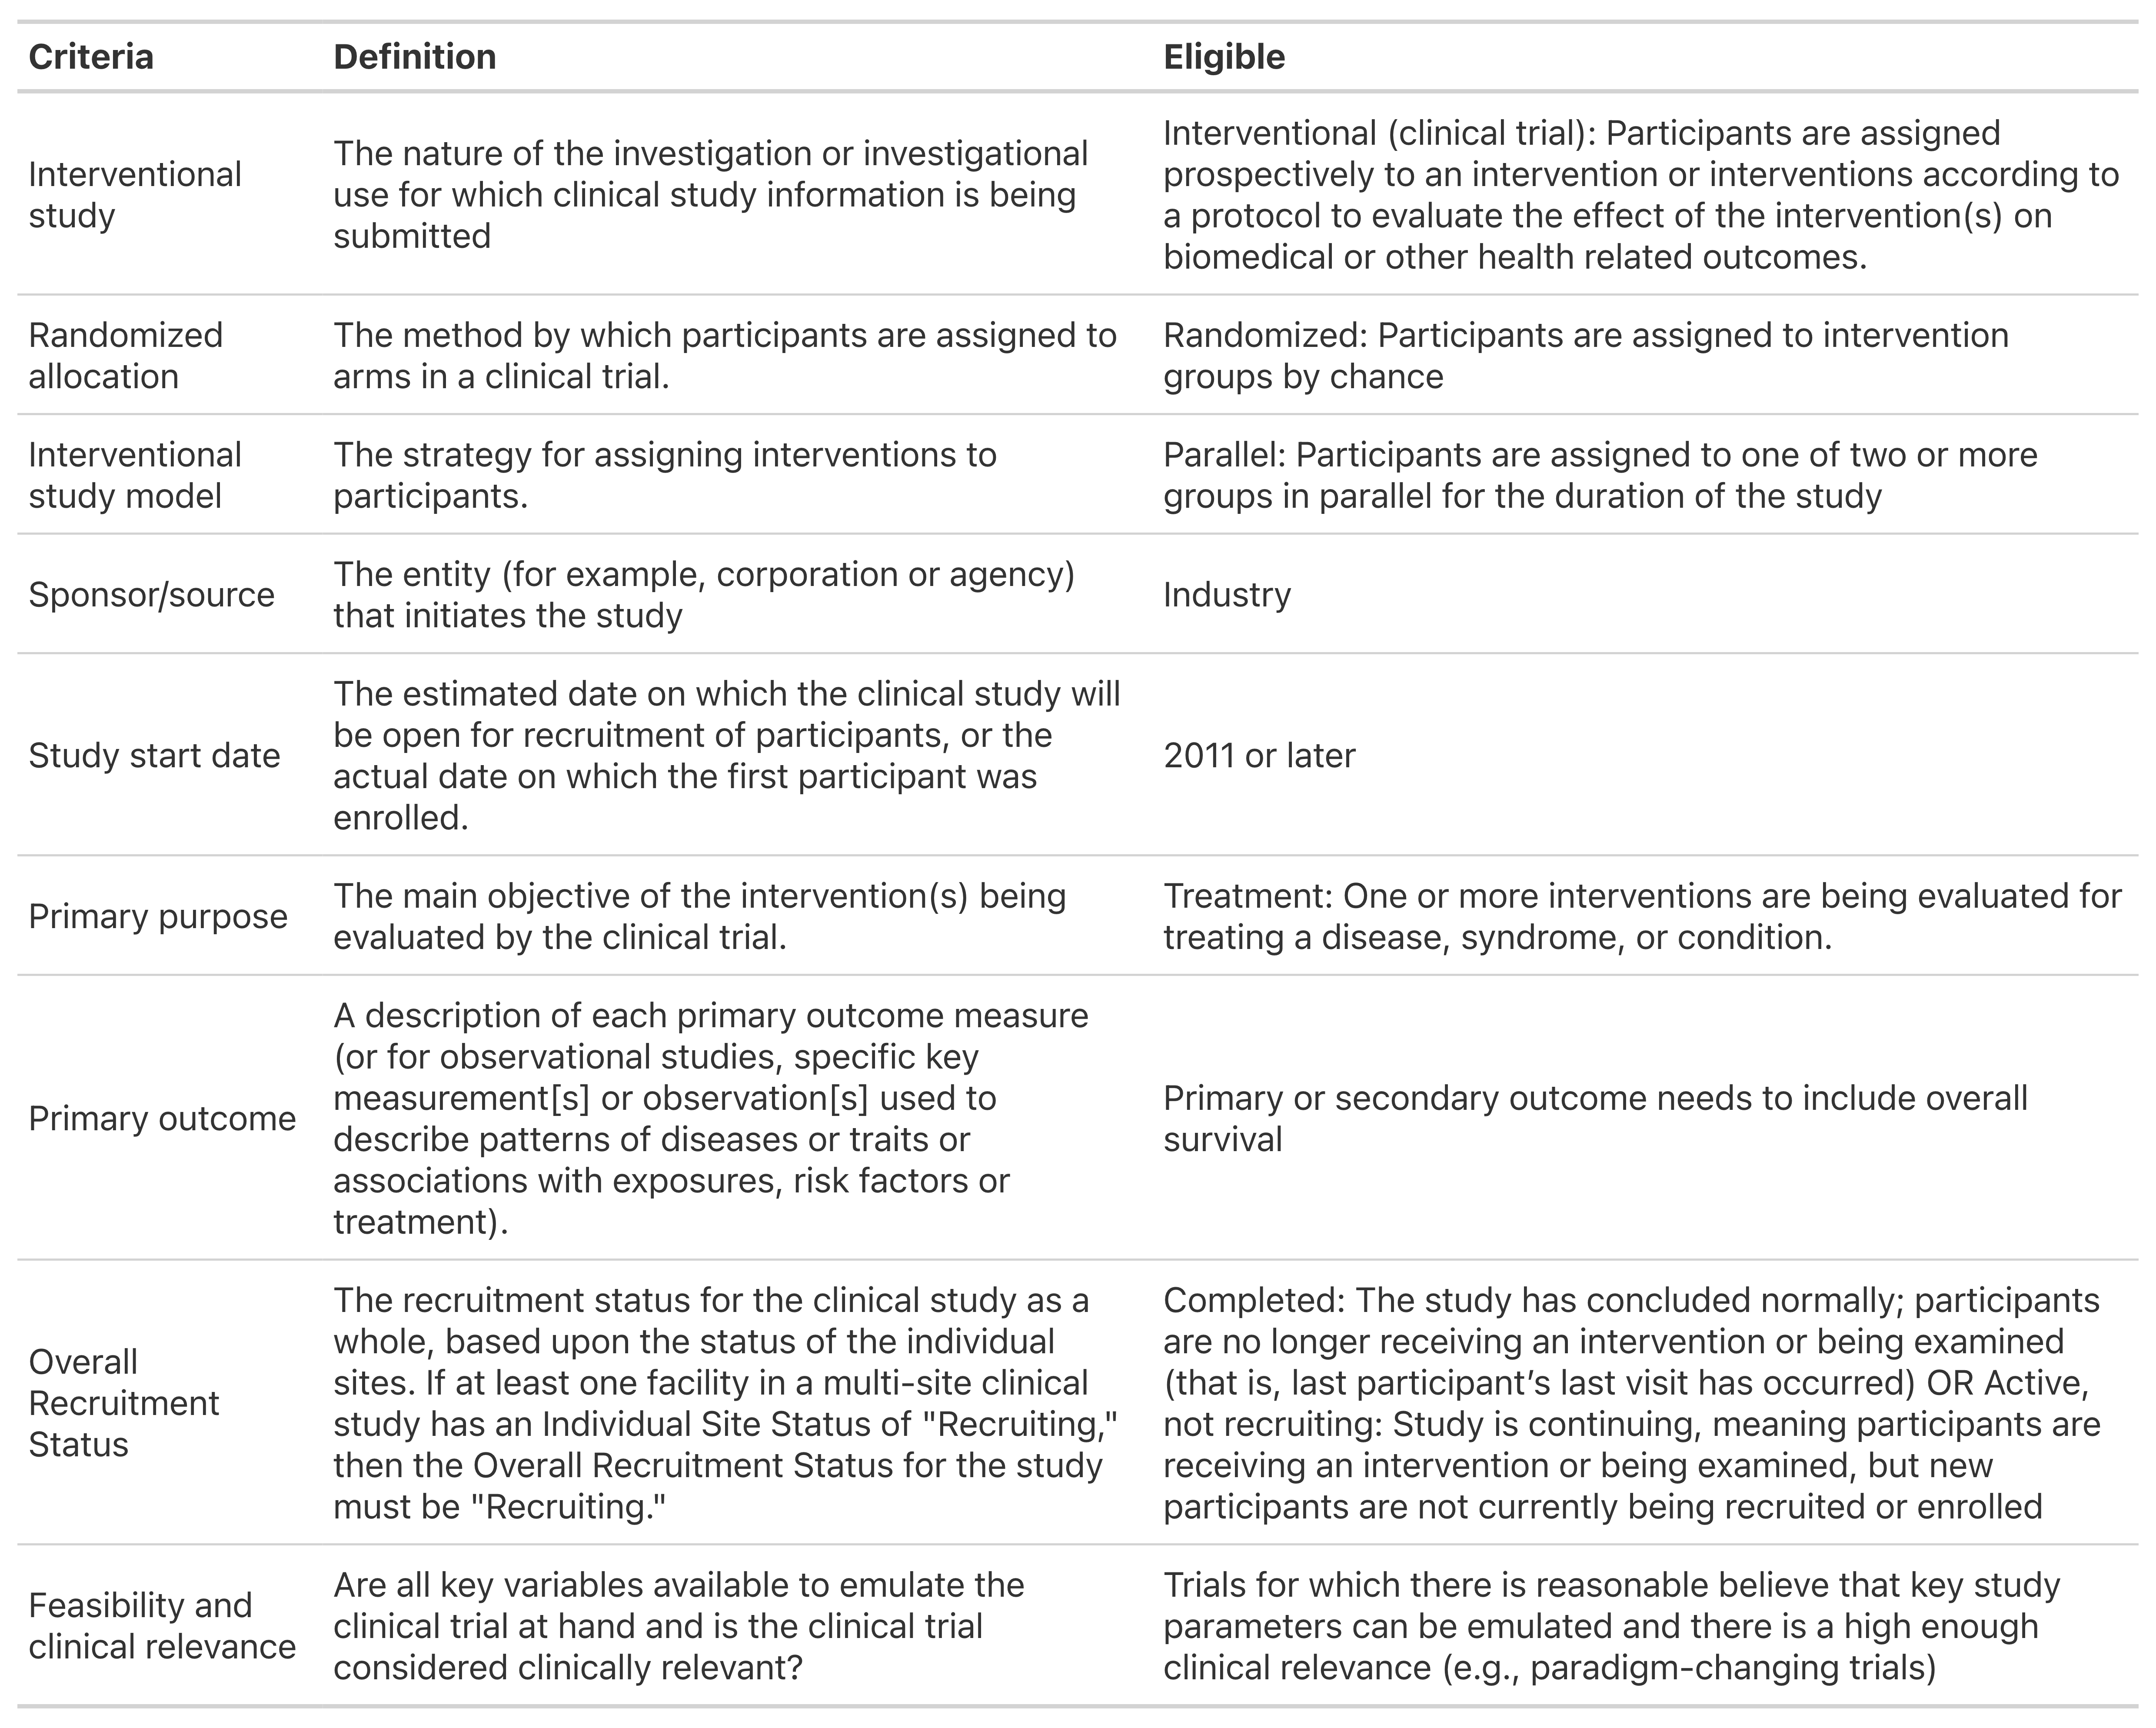
\includegraphics[keepaspectratio]{../tables/Table_1_trial_eligibility.png}}

}

\end{table}%

\newpage{}

\begin{table}[h]

\caption{\label{tbl-rcts}Tentative list of randomized controlled trials
(RCTs) considered for emulation.}

\centering{

\pandocbounded{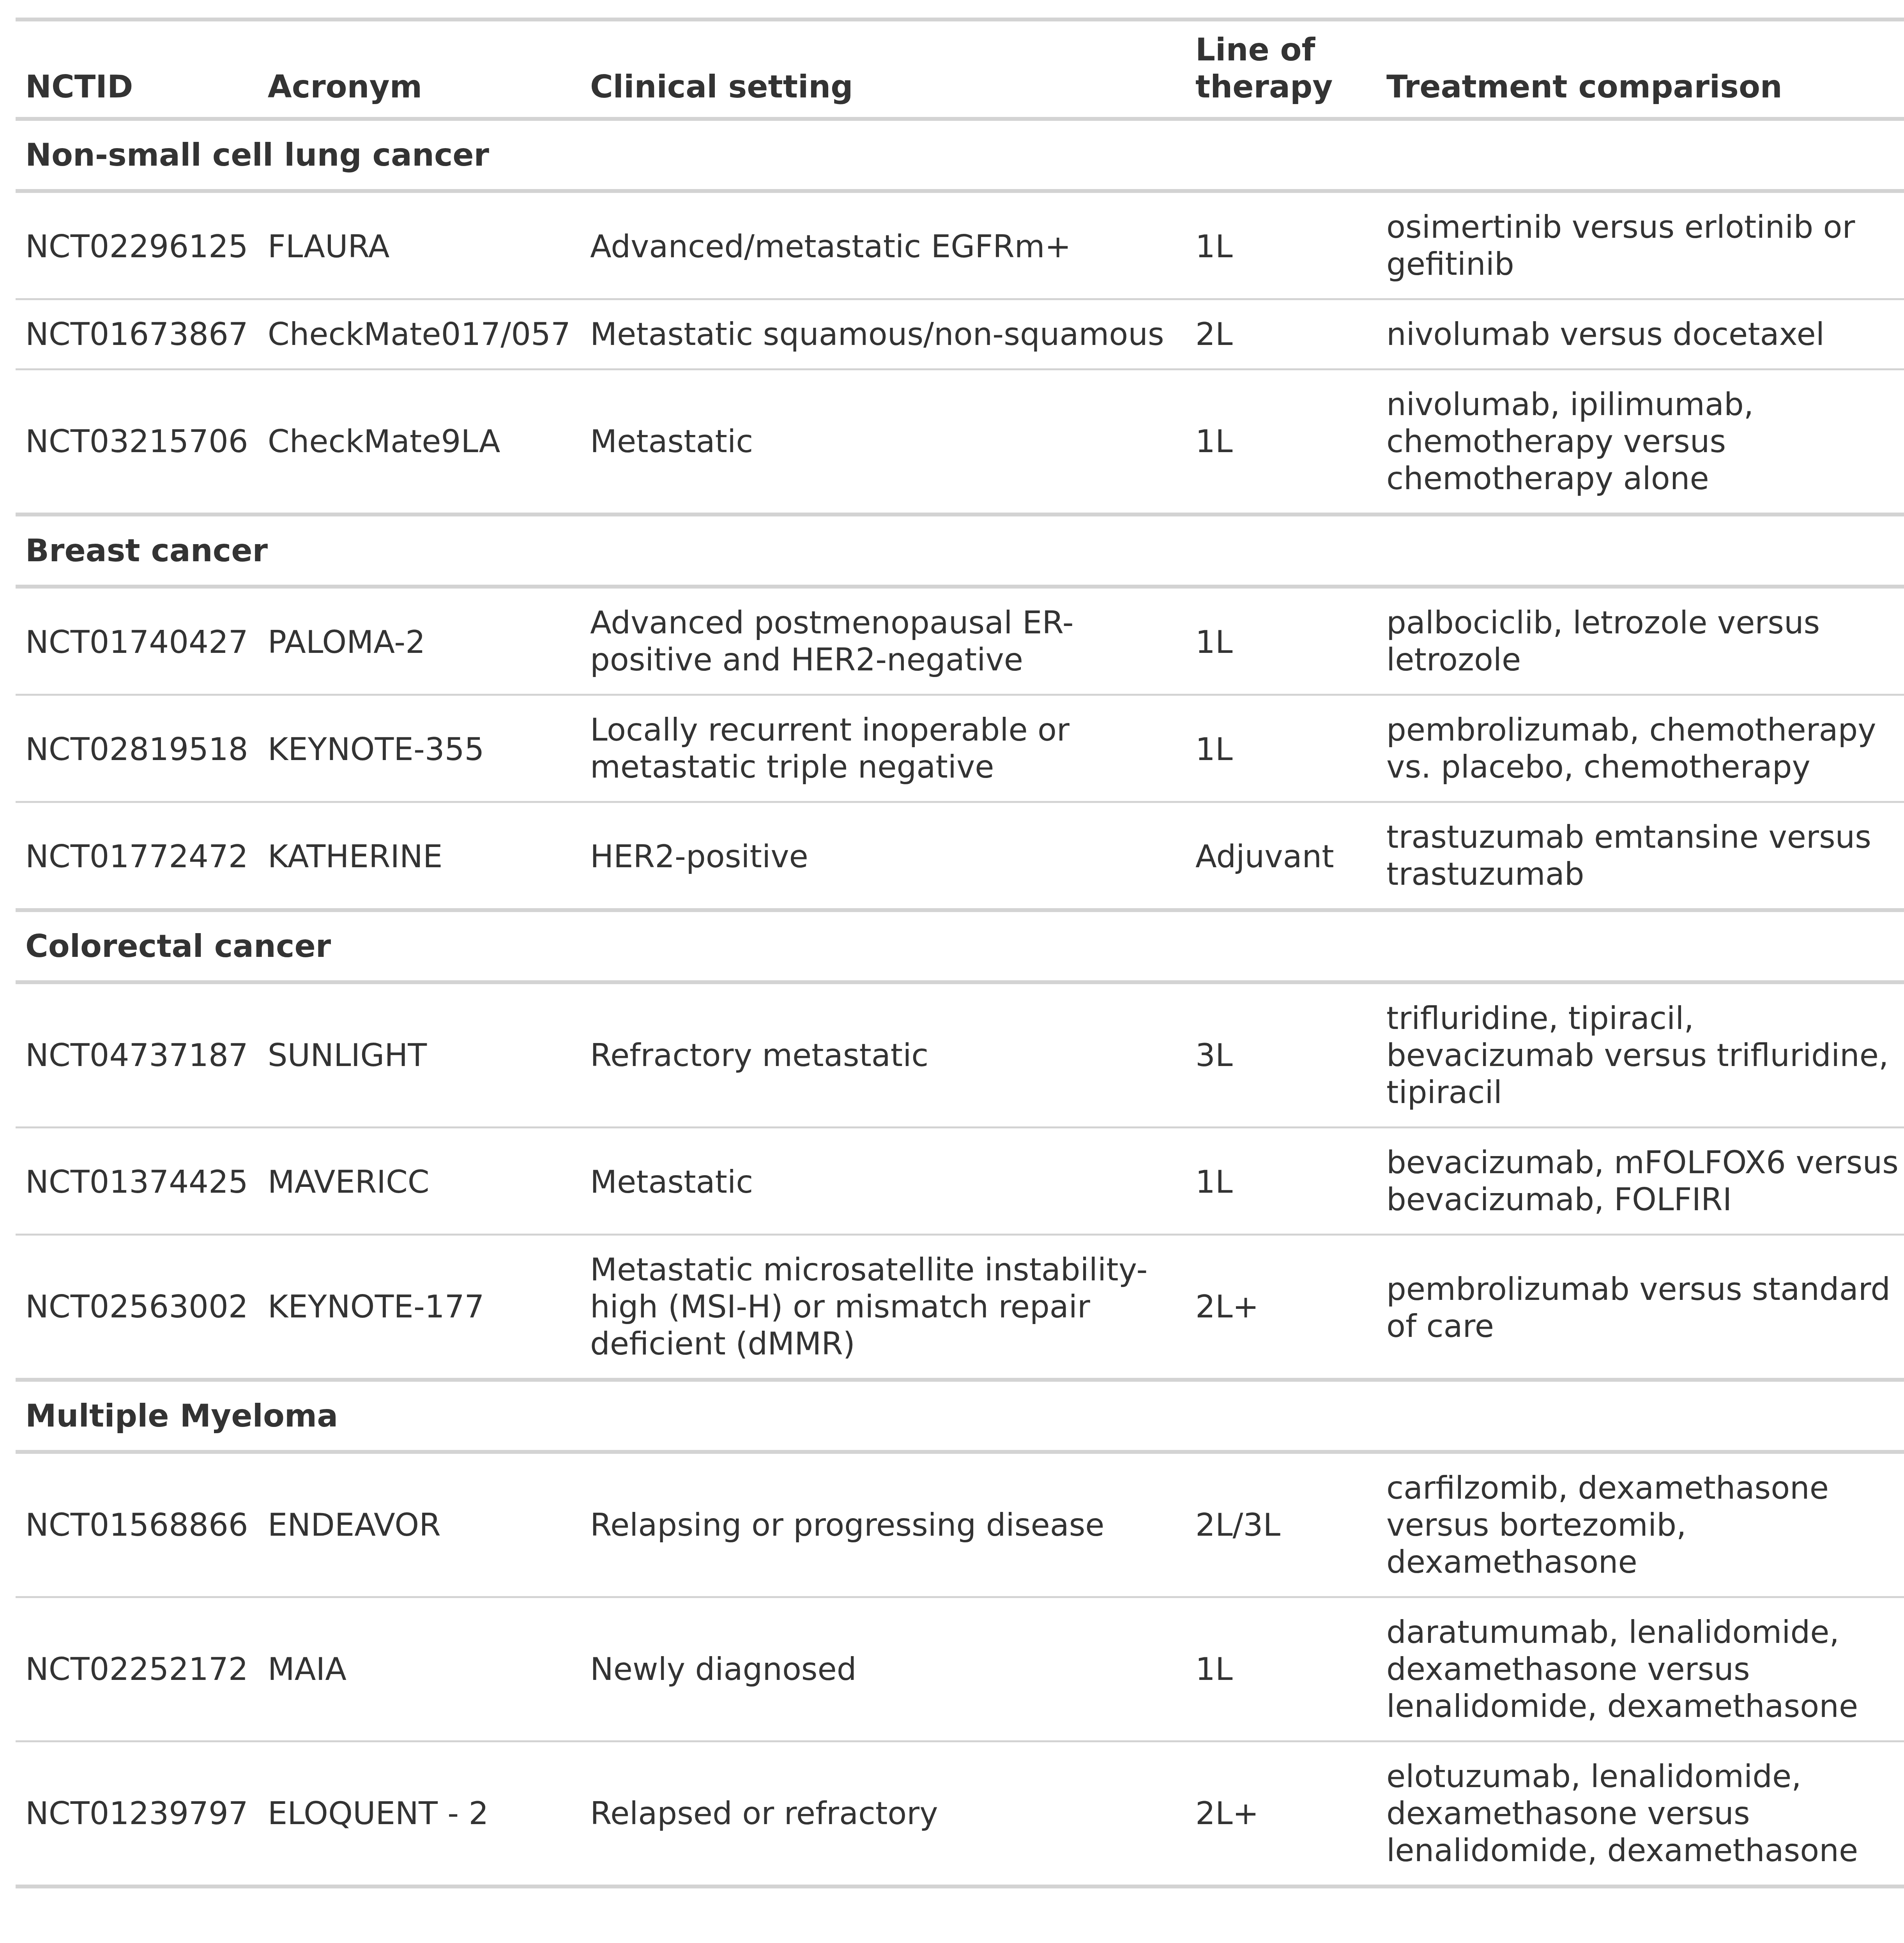
\includegraphics[keepaspectratio]{../tables/Table_2_trial_selection.png}}

}

\end{table}%

\newpage{}

\begin{table}[h]

\caption{\label{tbl-metrics}Example visualization of agreement metrics.}

\centering{

\pandocbounded{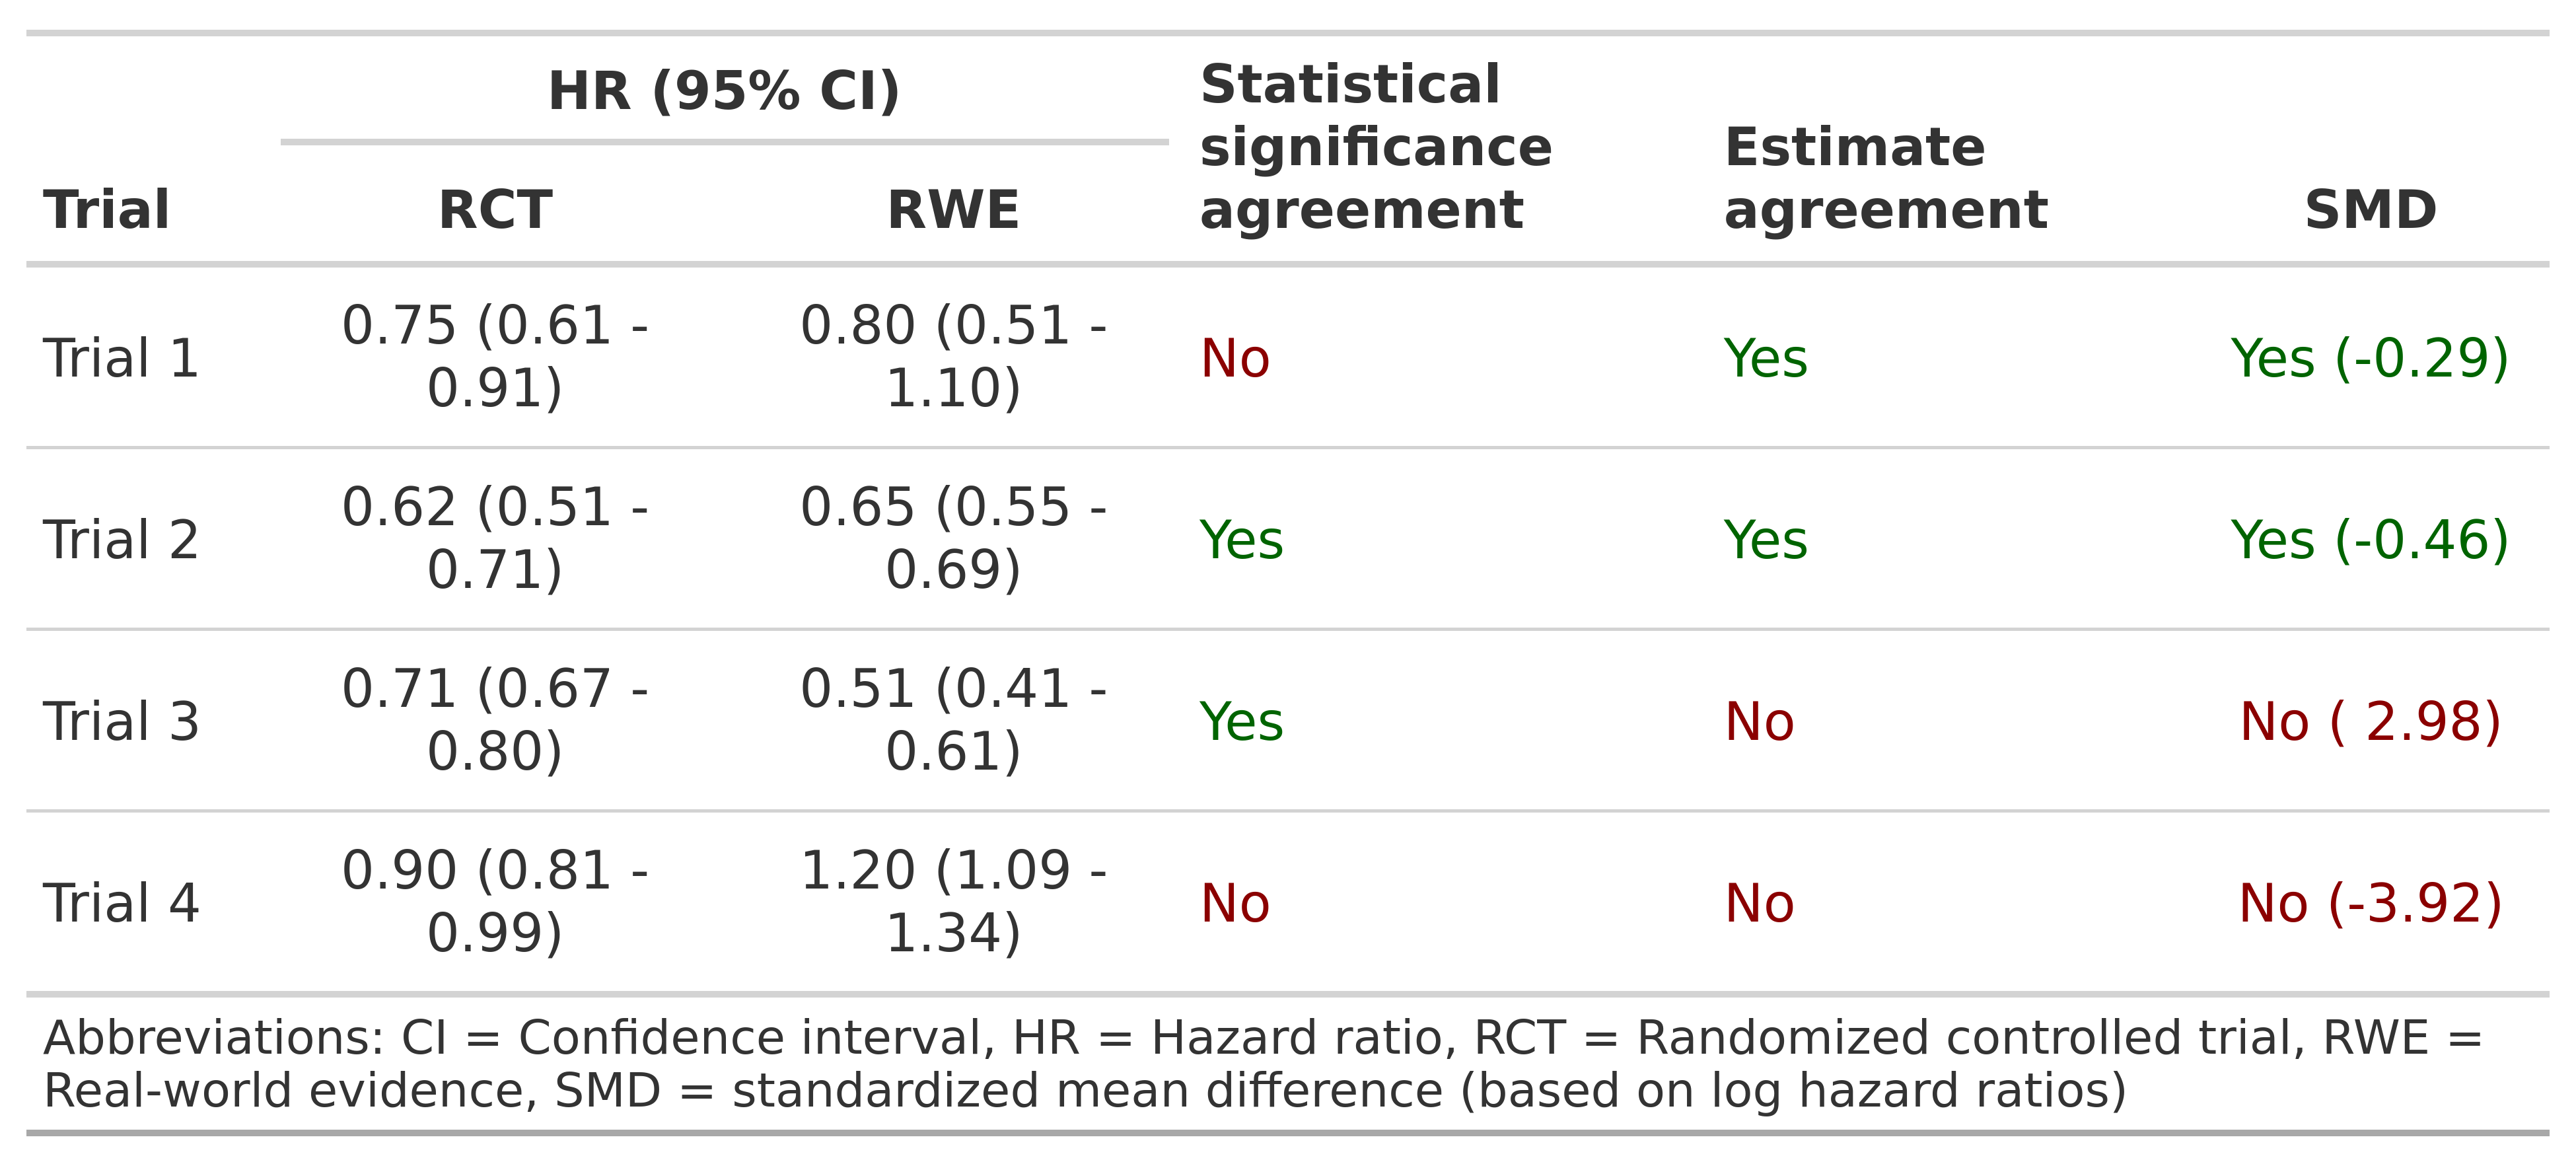
\includegraphics[keepaspectratio]{../tables/Table_3_agreement_metrics.png}}

}

\end{table}%

\newpage{}

\section*{Figures}\label{figures}
\addcontentsline{toc}{section}{Figures}

\begin{figure}[h]

\caption{\label{fig-process}Systematic process to understand
effectiveness claims of oncology trials using real-world evidence.}

\centering{

\pandocbounded{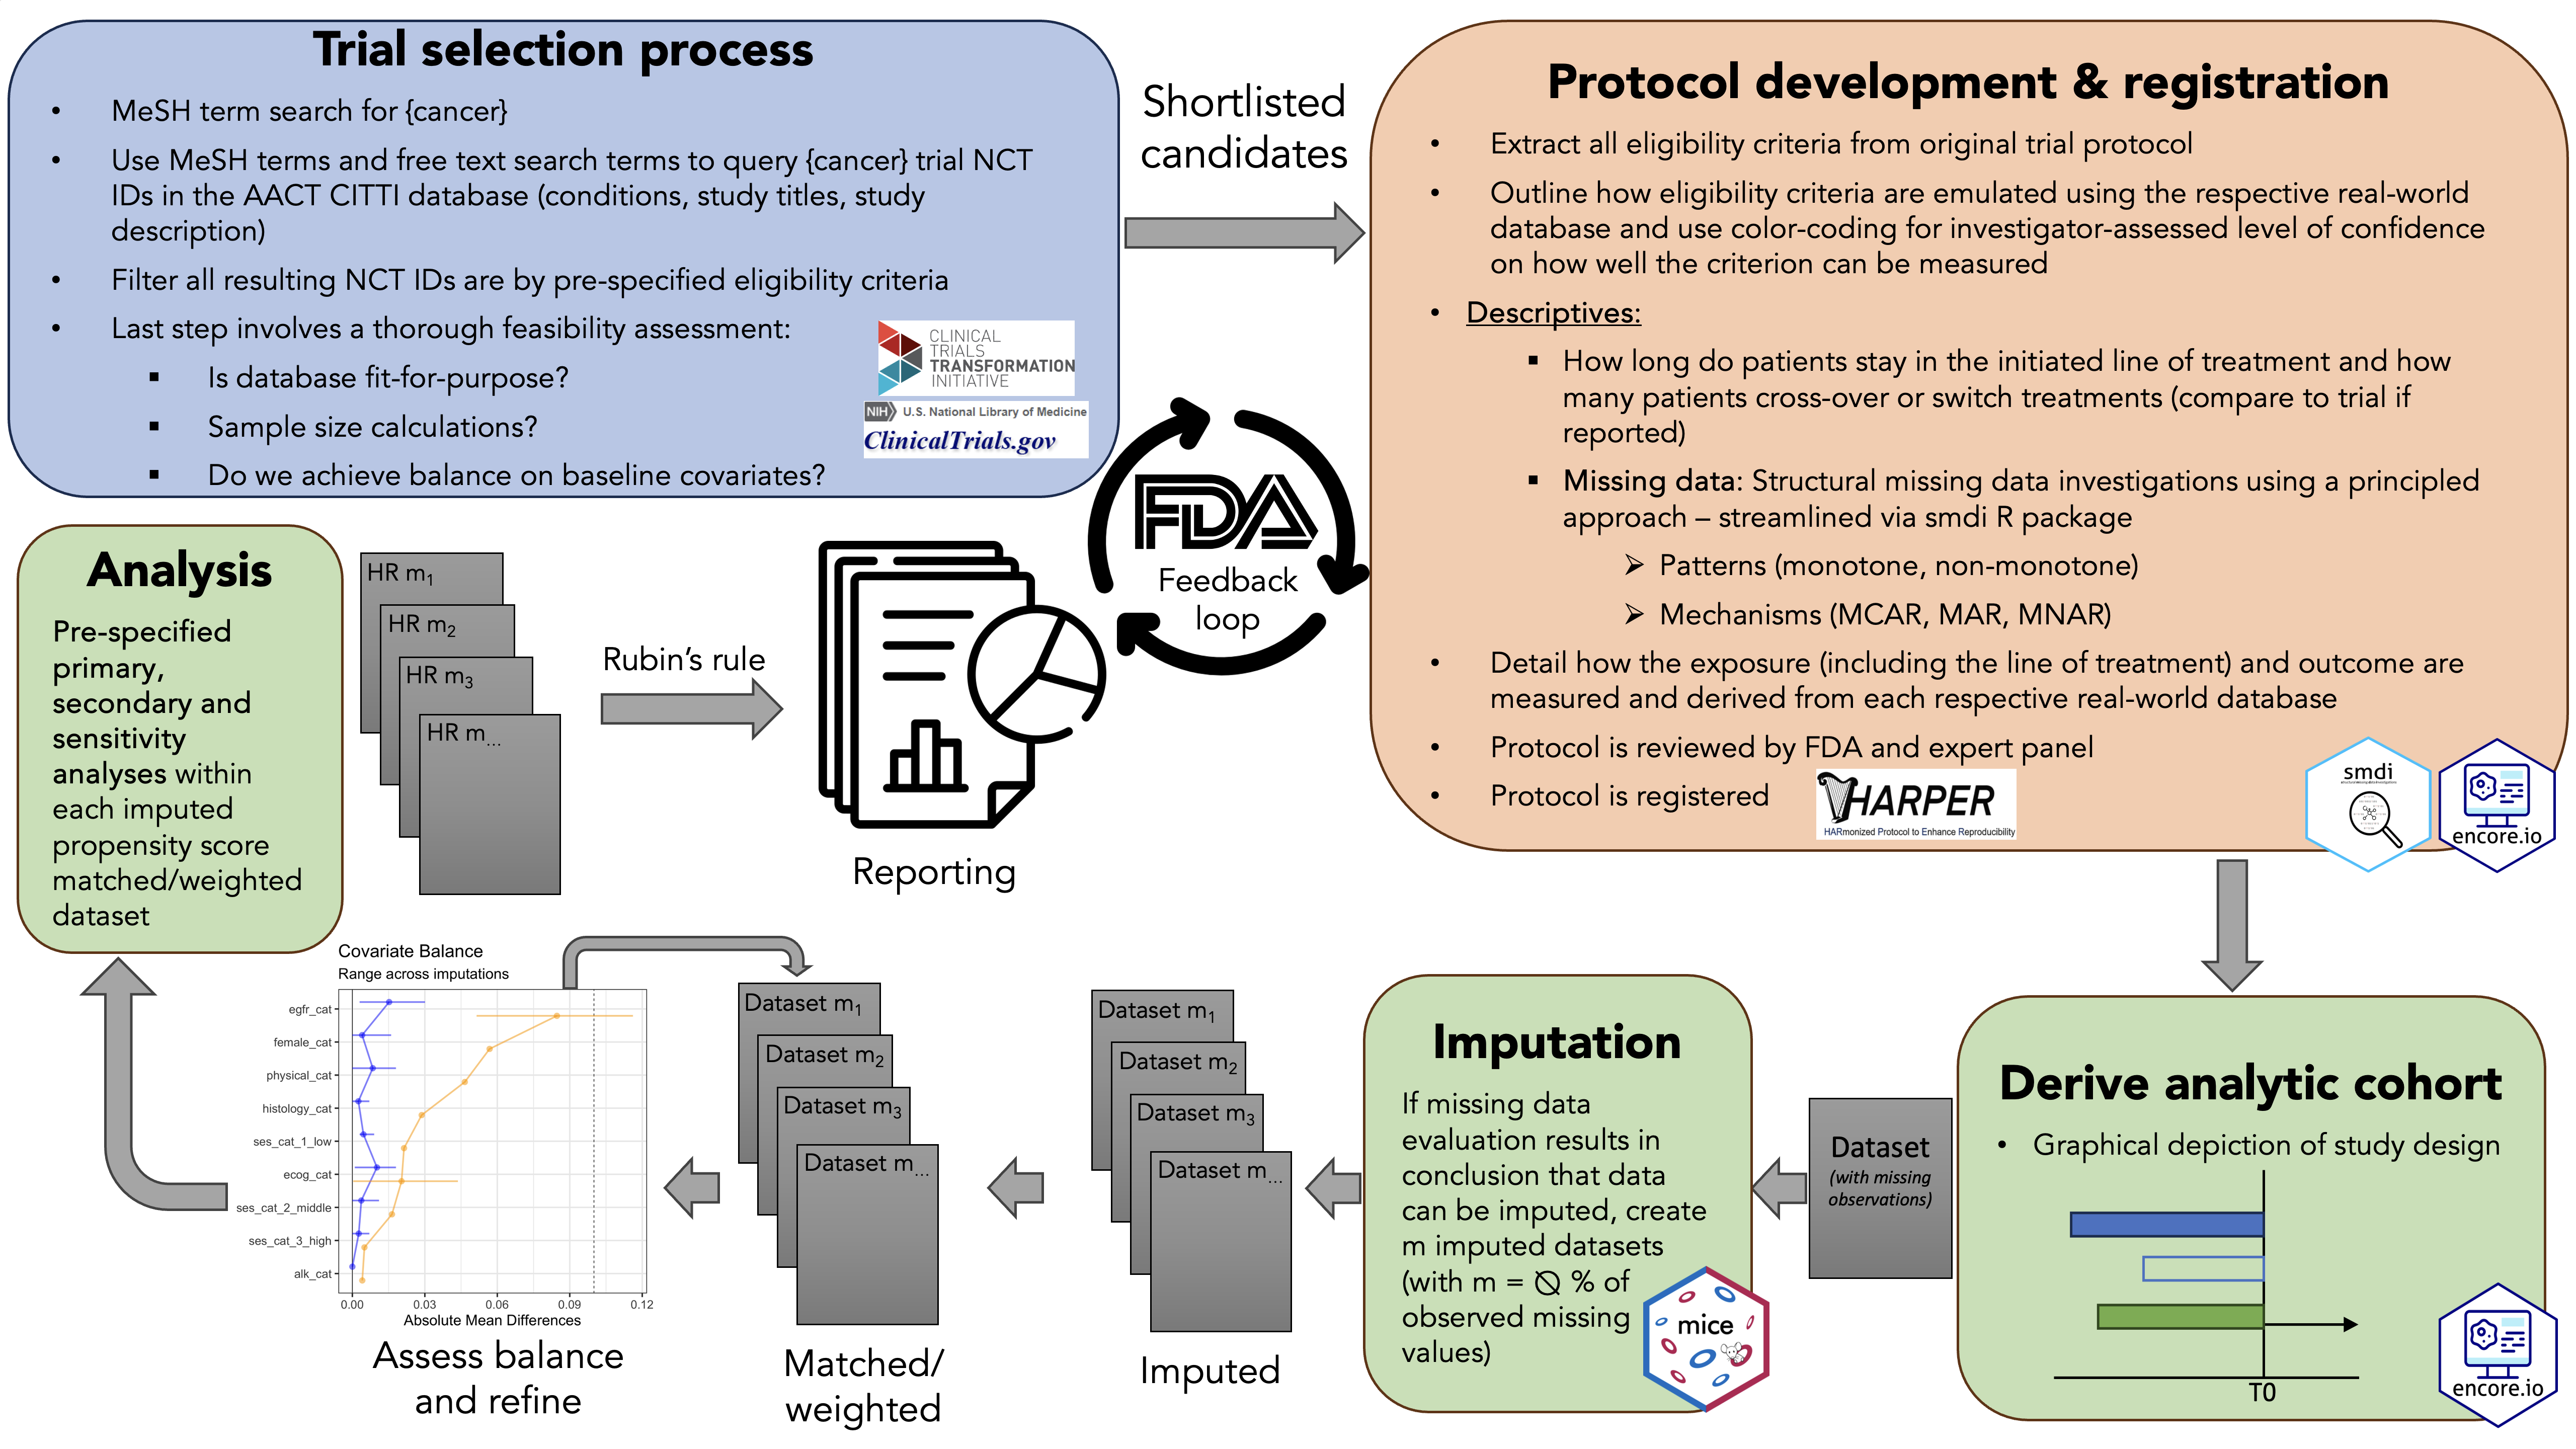
\includegraphics[keepaspectratio]{../figures/process.png}}

}

\end{figure}%

\newpage{}

\begin{figure}[h]

\caption{\label{fig-initiators}Example visualization of descriptive drug
utilization analyses displaying a) initiation trends between compared
regimens based on calendar time, b) cumulative rate of patients
switching to another line of treatment.}

\centering{

\pandocbounded{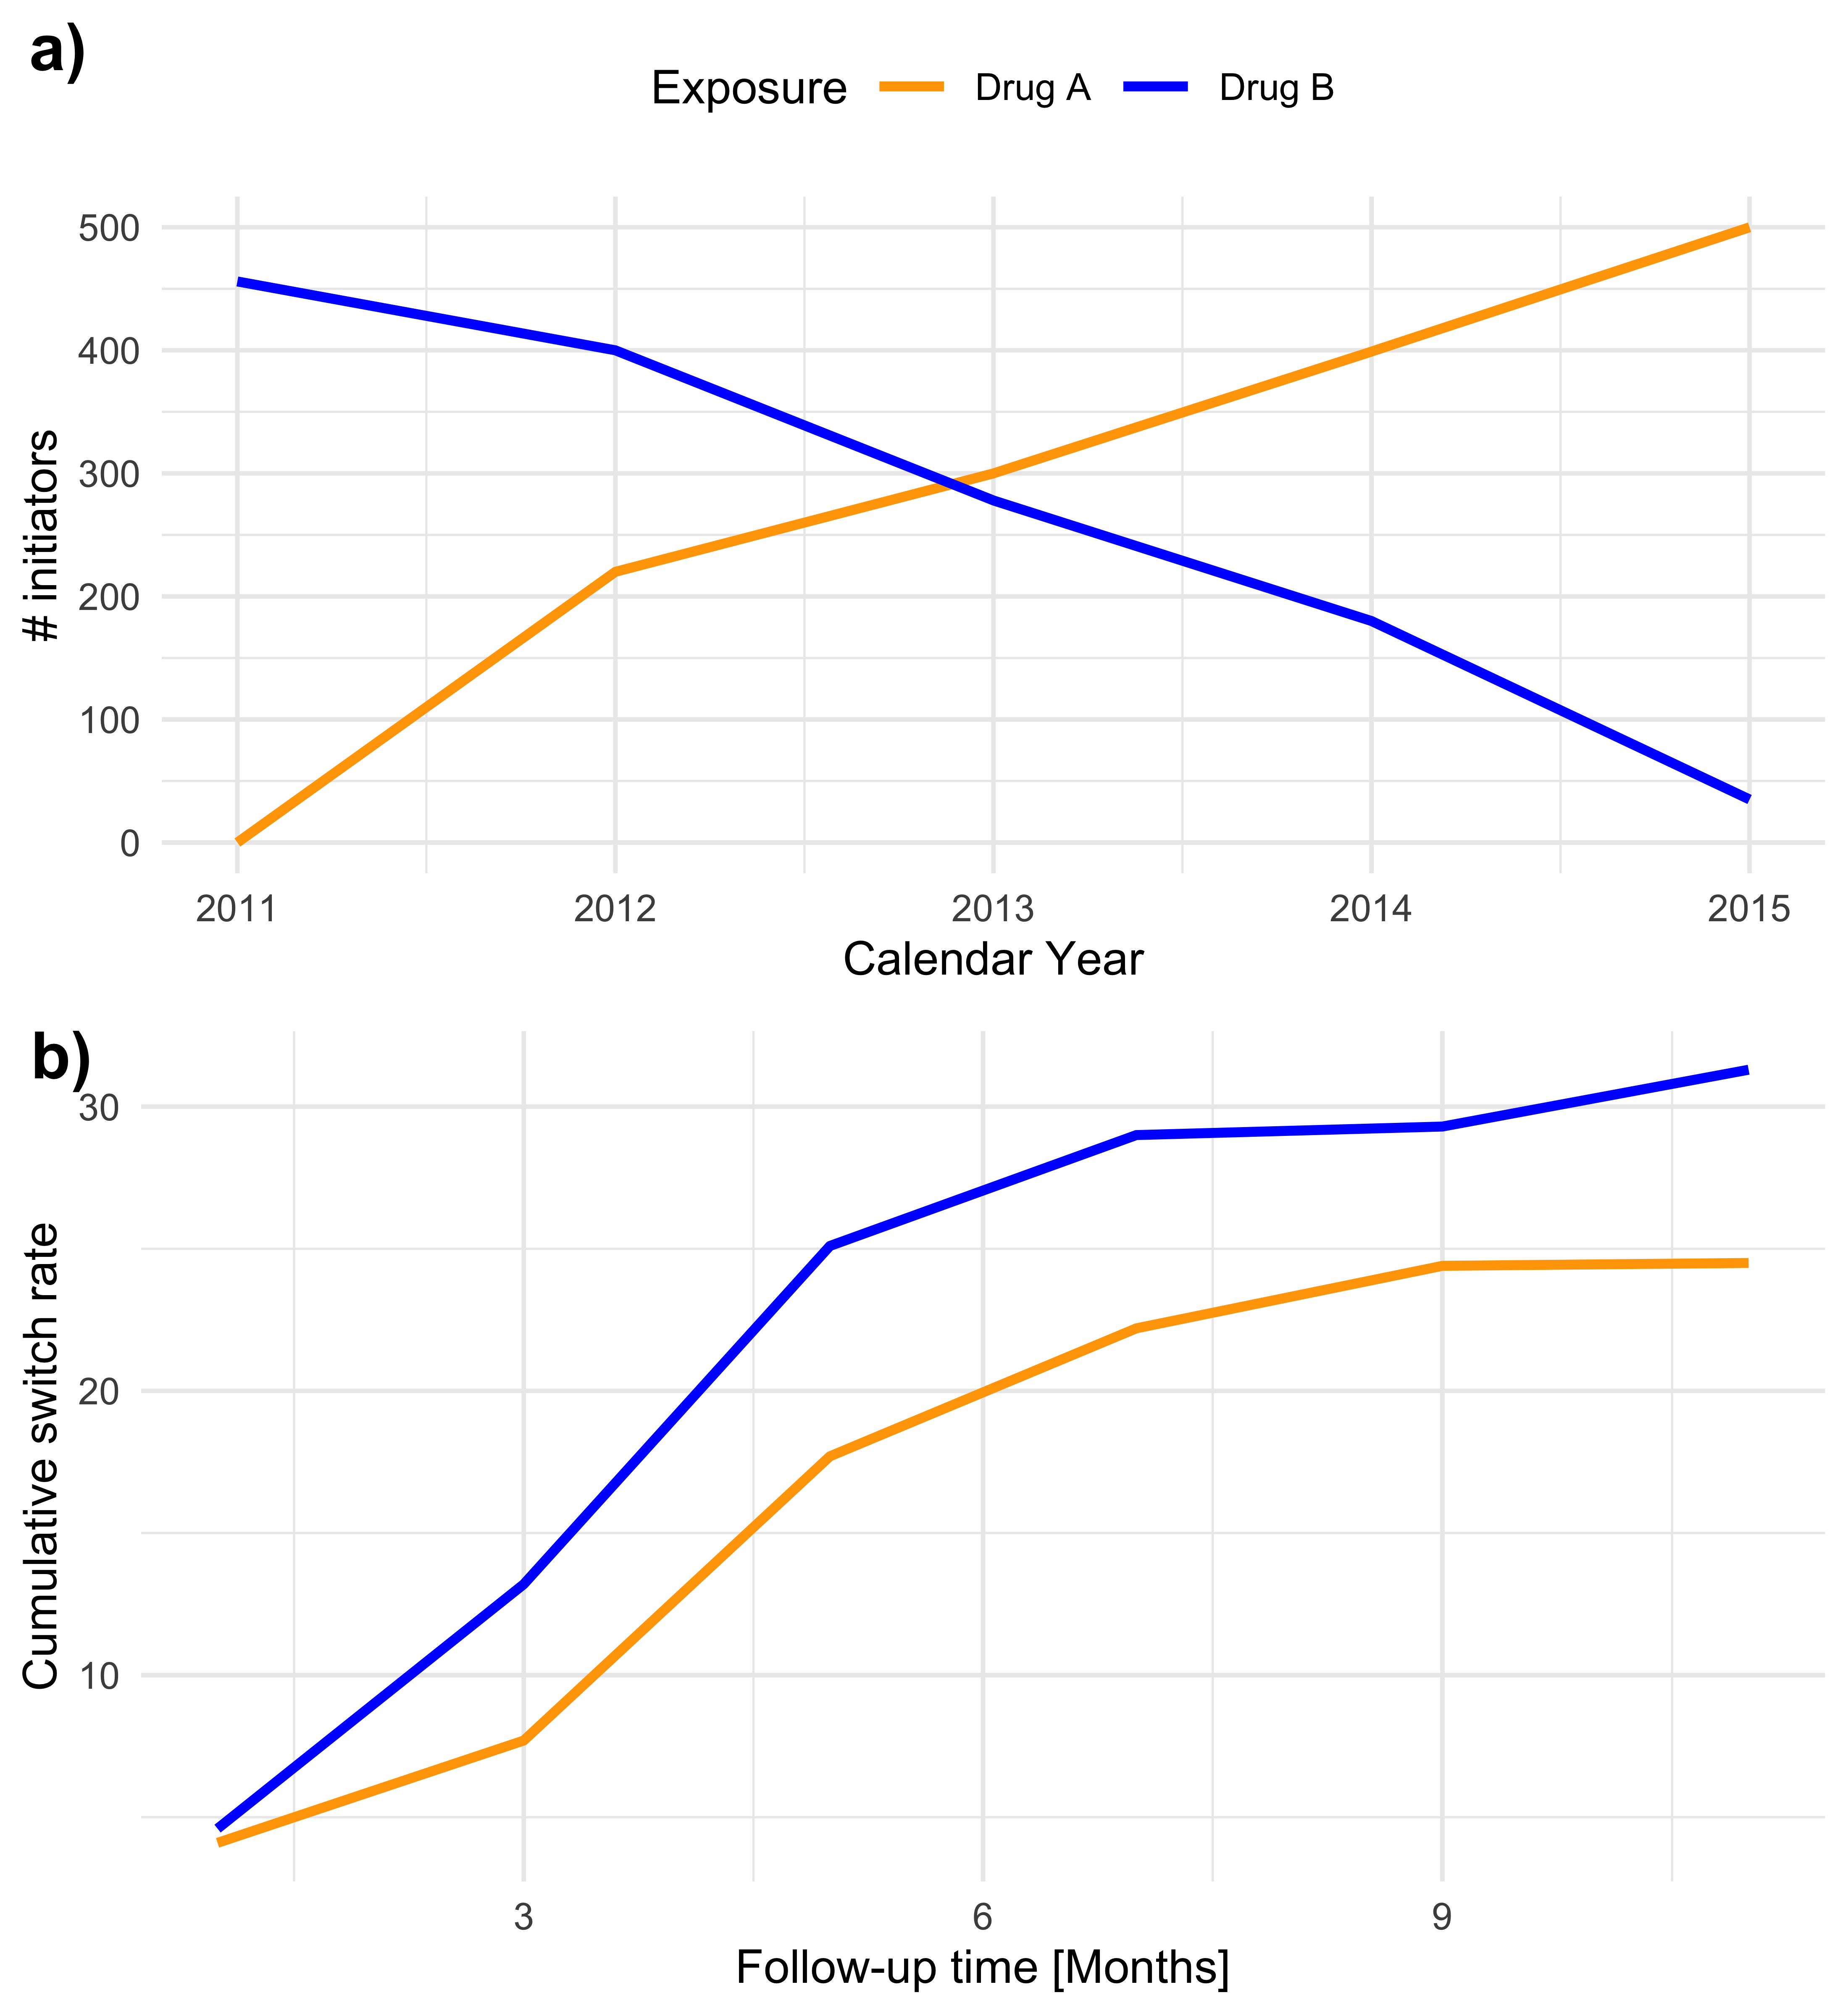
\includegraphics[keepaspectratio]{Figure_2_utlization.png}}

}

\end{figure}%

\newpage{}

\begin{figure}[h]

\caption{\label{fig-balance}Assessment of a) covariate balance and b)
distributional balance of a prognostic score for overall survival before
and after propensity score matching or weighting across multiple imputed
datasets.}

\centering{

\pandocbounded{\includegraphics[keepaspectratio]{Figure_3_balance.png}}

}

\end{figure}%




\end{document}
